% numerical.tex

\cleardoublepage
\chapter{Optimised Ascent Trajectory}\label{chapter:Ascent}

This chapter presents a maximum payload-to-orbit trajectory optimisation for the rocket-scramjet-rocket launch system incorporating the SPARTAN scramjet-powered accelerator. 
This launch system is simulated being launched from the Equatorial Launch Australia launch site in East Arnhem Land (Detailed in Section \ref{sec:mission}), and delivers a small satellite into sun synchronous orbit. LODESTAR is used to calculate maximum payload-to-orbit trajectory solutions for a variety of mission profiles.
First, a trajectory is calculated for the case in which the SPARTAN flies at constant dynamic pressure. This trajectory is calculated to serve as a baseline for comparisons to be made, as previous studies have assumed that flying the SPARTAN at its maximum allowable dynamic pressure would produce the best overall system performance[CITEXX]. An optimal payload-to-orbit trajectory is then developed, and the trajectory shape compared and contrasted to the constant dynamic pressure trajectory.
Lastly, a sensitivity study is performed, varying key performance parameters of the launch system and investigating the effects of each parameter on the performance of the launch system. 

The following trajectories are developed: 
\begin{enumerate}
	\item: Case 1: $q = $ 50kPa fixed SPARTAN trajectory with minimum pull-up. \newline$\rightarrow$ This trajectory provides a baseline trajectory for comparison purposes.
	\item: Case 2: Trajectory optimised for payload-to-orbit, $q_{max} = $ 50kPa. \newline$\rightarrow$ This trajectory demonstrates improved performance through trajectory optimisation.
	\item: Case 3: Variation of maximum allowable dynamic pressure between $q_{max} = $ 40kPa \& $q_{max} = $ 60kPa. 
	\newline$\rightarrow$ Comparison of these simulations allows an investigation into the influence of the SPARTAN's ability to withstand aerodynamic forces on the performance of the launch vehicle.
	\item: Case 4: Variation of the coefficient of drag of the SPARTAN between $C_d = 90\%$ \& $C_d = 110\%$. 
	\newline$\rightarrow$ Comparison of optimal trajectories with drag variation allows investigation of the effects of variations and uncertainties in the SPARTAN's aerodynamic design on launch system performance.
	\item: Case 5: Variation of the specific impulse of the SPARTAN's C-REST engines between $I_{SP} = 90\%$ \& $I_{SP} = 110\%$. 
	\newline$\rightarrow$ Comparison of optimal trajectories with specific impulse variation allows investigation of the effects of the efficiency of the C-REST engines on the performance of the launch system. 
	\item: Case 6: Variation of the mass of the SPARTAN between $m_2 = 90\%$ \& $m_2 = 110\%$. 
	\newline$\rightarrow$ Comparison of optimal trajectories with SPARTAN mass variation allows investigation of the effects of the internal design of the SPARTAN on the launch system performance. 
	\item: Case 7: Variation of the fuel mass of the SPARTAN between $m_{fuel} = 90\%$ \& $m_{fuel} = 110\%$. 
	\newline$\rightarrow$ Comparison of optimal trajectories with SPARTAN fuel mass variation allows investigation of the effects of the amount of fuel which the SPARTAN is able to carry on the launch system efficiency. 
	\item: Case 8: Variation of the mass of the third stage rocket between $m_3 = 90\%$ \& $m_3 = 110\%$. 
	\newline$\rightarrow$ Comparison of optimal trajectories with third stage mass variation allows investigation of the effects of the third stage internal layout on the efficiency of the system. 
	\item: Case 9: Variation of the thrust of the third stage rocket between $T_3 = 90\%$ \& $T_3 = 110\%$. 
	\newline$\rightarrow$ Comparison of optimal trajectories with third stage thrust variation allows investigation of the effects of the output of the third stage engine on the efficiency of the launch system. 
	\item Case 10: Variation of the coefficient of drag of the third stage rocket between $C_d = 90\%$ \& $C_d = 110\%$.
	\newline$\rightarrow$ Comparison of optimal trajectories with third stage drag variation allows investigation of the effects of variations and uncertainties in the aerodynamic design of the third stage on the performance of the launch system.
\end{enumerate}
These case studies allow the benefits of flying an optimised trajectory to be quantified, and enable the key design parameters of the SPARTAN and third stage rocket to be characterised. Comparisons between the cases allows for the relative impact of each design parameter on the payload-to-orbit, as well as on the performance of each individual stage, to be assessed. 
In order to effectively compare the performance of the stages of the launch system, exergy analysis is utilised. Exergy expresses how much useful work is available to a system, and exergy efficiency quantifies how well a system utilises the available work. Exergy is lost due to inefficiencies within a launch system. These inefficiencies arise from many sources, including the energy being lost due to the inability of the propulsion system to convert all of the combustion energy to thrust, the energy which must be used to overcome drag, and energy being lost due to manoeuvring. Exergy efficiency is an important parameter for analysing launch vehicles, allowing the relative efficiencies of each stage to be compared when the design or trajectory of a launch system is varied[CITEXX]. The exergy efficiency of a stage of a launch system is expressed as the fraction of the fuel combustion energy which is turned into kinetic and potential energy during flight:
\begin{equation}
\eta_{exergy,stage} = 1 - \frac{\Delta m_{fuel}H_{fuel} - \Delta KE - \int mg dz}{\Delta m_{fuel}H_{fuel}},
\end{equation}
where $H_{fuel}$ is the heating value of the fuel, $KE$ is the change in the kinetic energy of the stage, and $\int mg dz$ is the change in potential energy of the stage over its trajectory.
\nomenclature{$H$}{Heating Value (J/kg)}
\nomenclature{$KE$}{Kinetic Energy (J)}
\nomenclature{$PE$}{Potential Energy (J)}
This exergy efficiency expresses how efficiently each stage utilises its available fuel over each individual trajectory, but does not account for the effects of the unused mass of each stage on the performance of the launch system. The total exergy efficiency of the launch system is calculated as the fraction of the total available energy which goes directly into placing the payload into orbit:
\begin{equation}
\eta_{exergy} = \frac{\Delta KE_{payload} + \Delta PE_{payload}}{\sum_{stage} \Delta m_{fuel}H_{fuel}}.
\end{equation}
This total exergy efficiency expresses how efficiently the launch system as a whole is able to accelerate the payload to orbit. 

\textcolor{red}{need to mention that the exergy can be affected by the amount of fuel (as its variable), and kee this is mind during discussion. -i dont think using specific exergy is  useful though}

\section{Case 1: Constant Dynamic Pressure Trajectory}
\begin{figure}[ht]
	\centering
	\includegraphics[width=1\linewidth]{../LODESTAR_FINAL/Results/mode900/GroundTrackConstq}
	\caption{Maximum payload-to-orbit trajectory path with the SPARTAN flying at constant dynamic pressure (Case 1). Initial heading angle 92.6$^\circ$.}
	\label{fig:GroundTrackConstq}
\end{figure}

The first trajectory which is produced using LODESTAR is a maximum payload-to-orbit trajectory in which the SPARTAN flies a constant dynamic pressure path, at its maximum allowable dynamic pressure of 50kPa. In order to drive the SPARTAN towards a constant dynamic pressure path, the cost function described in Table \ref{tab:SPARTANascentsetup} is utilised. In addition to the dynamic pressure cost function, the maximum payload-to-orbit cost function is also active on the third stage phase, so that when the SPARTAN is close to 50kPa, the third stage will fly a maximum payload-to-orbit trajectory from the termination of the SPARTAN's constant dynamic pressure path.
Previous studies have assumed that flying the SPARTAN at constant dynamic pressure will produce the best possible system performance [CITEXX]. Because of this assumption, a constant dynamic pressure trajectory is produced to serve as a baseline for comparison with the maximum payload-to-orbit optimised trajectory. Producing a constant dynamic pressure trajectory also serves to verify that LODESTAR is able to calculate a trajectory in which the SPARTAN flies at the maximum possible dynamic pressure for the duration of its flight. 
The aerodynamics and design of the launch system have been updated in this study[CITEXX], with the use of Cart3D for aerodynamic calculations, the additional of fuel mass to the SPARTAN, an updated third stage design, and the addition of a first stage. Due to these changes it must be confirmed that the system is able to fly a constant dynamic pressure path, to ensure that any deviations from a constant dynamic pressure path in the payload-to-orbit optimised trajectory serve to improve the performance of the system, rather than being a result of the problem setup or design constraints. 

\begin{table}[ht]
	\centering
	
	\begin{tabular}{l c } 
		\hline \textbf{Trajectory Condition}
		& Constq

		\\
		\hline \textbf{Payload to Orbit (kg)}
		& \textbf{\PayloadToOrbitConstq}
		\\
		\textbf{Total $\eta_{exergy}$ (\%)}
		& \textbf{\totalExergyEffConstq}
		\\
		\hline 
		\textbf{1$^{st}$ Stage $\eta_{exergy}$ (\%)}
		& \textbf{\firstExergyEffConstq}
		\\
		\textbf{Separation Alt, 1$\rightarrow$2 (km)}
		& \firstsecondSeparationAltConstq
		\\
		\textbf{Separation v, 1$\rightarrow$2 (m/s)}
		& \firstsecondSeparationvConstq
		\\
		\textbf{Separation $\gamma$, 1$\rightarrow$2 (m/s)}
		& \firstsecondSeparationgammaConstq
		\\
		\hline 
		\textbf{2$^{nd}$ Stage $\eta_{exergy}$ (\%)}
		& \textbf{\secondExergyEffConstq}
		\\
		\textbf{Separation Alt, 2$\rightarrow$3 (km)}
		& \secondthirdSeparationAltConstq
		\\
		\textbf{Separation $v$, 2$\rightarrow$3 (m/s)}
		& \secondthirdSeparationvConstq
		\\
		\textbf{Separation $\gamma$, 2$\rightarrow$3 (deg)}
		& \secondthirdSeparationgammaConstq
		\\
		\textbf{Separation $q$, 2$\rightarrow$3(kPa)}
		& \secondthirdSeparationqConstq
		\\
		\textbf{2$^{nd}$ Stage L/D, 2$\rightarrow$3}
		& \secondthirdSeparationLDConstq
		\\
		\textbf{2$^{nd}$ Stage Flight Time (s)}
		& \secondFlightTimeConstq
		\\
		\hline 
		\textbf{3$^{rd}$ Stage $\eta_{exergy}$ (\%)}
		& \textbf{\thirddExergyEffConstq}
		\\
		\textbf{3$^{rd}$ Stage $t$, $q >$ 5kpa (s)}
		& \thirdqOverFiveConstq
		\\
		\textbf{3$^{rd}$ Stage max $\alpha$ (deg)}
		& \thirdmaxAoAConstq
		\\
		\textbf{3$^{rd}$ Stage Fuel Mass (kg)}
		& \thirdmFuelConstq
		\\
		\hline 
	\end{tabular} 
	
	\caption{}
	\label{tab:constqsummary}
\end{table}
\begin{figure}[ht!]
	\centering
	\includegraphics[width=0.9\linewidth]{../LODESTAR_FINAL/Results/mode900/FirstStageConstq}
	\caption{The first stage trajectory of the launch system, with the SPARTAN constrained to flight at constant dynamic pressure (Case 1).}
	\label{fig:FirstStageConstq}
\end{figure}
LODESTAR is able to successfully simulate the trajectory of the rocket-scramjet-rocket system, with the SPARTAN flying at constant dynamic pressure, achieving a payload-to-orbit of \PayloadToOrbitConstq kg.
Figure \ref{fig:GroundTrackConstq} shows the simulated trajectory path, and Table \ref{tab:constqsummary} provides a summary of the key parameters of the trajectory, including the exergy efficiency of each stage.


The rocket-scramjet-rocket system launches vertically, flying a fixed vertical trajectory for 3.9s, after which a pitchover is initiated at a heading angle of 92.6$^\circ$. Under power of the first stage rocket, the launch system begins pitching, flying north-west, over the Arafura Sea. 
After pitchover the angle of attack stays constant at 0$^\circ$ for 49.1s, as shown in Figure \ref{fig:FirstStageConstq}. At this point, the angle of attack is reduced, reaching a minimum of -4.89$^\circ$, before increasing back up to 0$^\circ$ for stage separation. 
The SPARTAN is separated at a trajectory angle of \firstsecondSeparationgammaConstq$^\circ$ at an altitude of \firstsecondSeparationAltConstq km, a total flight time of 120.9s, with a total ground distance of XXkm covered under power of the first stage rocket. 
 In order to release the SPARTAN at a lower trajectory angle, the first stage must launch with a lower fuel mass, to allow it to pitch in the correct manner. To achieve a constant dynamic pressure trajectory, the first stage launches with a fuel mass of 17010kg. This is significantly lower than the full amount of allowable fuel mass, 17934kg, indicating that the launch system is unable to achieve 50kPa first stage-SPARTAN conditions using the full fuel mass. 
The first stage rocket achieves an exergy efficiency of \firstExergyEffConstq \% when separating the SPARTAN onto a constant dynamic pressure trajectory. 


\begin{figure}[ht!]
\centering
\includegraphics[width=0.9\linewidth]{../LODESTAR_FINAL/Results/mode900/SecondStageConstq}
\caption{The constant dynamic pressure flight path of the SPARTAN (Case 1).}
\label{fig:SecondStageConstq}
\end{figure}


The constant dynamic pressure trajectory for the SPARTAN stage is shown in Figure \ref{fig:SecondStageConstq} with key results summarised in Table \ref{tab:constqsummary}. After the separation of the first stage rocket, the SPARTAN flies north west over the Arafura Sea, and crosses West Papua before releasing the third stage rocket. Due to the clear objective of a constant dynamic pressure trajectory, any deviations from the target dynamic pressure are readily apparent, allowing the efficacy of the optimiser to be verified. 
The constant dynamic pressure simulation, shown in Figure \ref{fig:SecondStageConstq}, shows very close adherence to 50kPa dynamic pressure (maximum 0.2\% deviation). Third stage release occurs at \secondFlightTimeConstq s at \secondthirdSeparationAltConstq km altitude. 
Over the trajectory, the Mach no. increases from 4.85 to 9.23, the velocity increases from \firstsecondSeparationvConstq m/s to \secondthirdSeparationvConstq m/s, and the flap deflection increases from $-3.2^\circ$ to $4.7^\circ$. At the beginning of the trajectory the equivalence ratio increases as the capture limitations are relaxed with increasing Mach number. This causes the net specific impulse to increase, to a maximum of 1481s, during the first 169.3s flight time.  After this initial increase, the net specific impulse ($I_{sp_{net}} = \frac{T-D}{\dot{m}_f g}$) decreases over the trajectory, as the efficiency of the scramjet engines decreases. 
The exergy efficiency of the SPARTAN is \secondExergyEffConstq \% over its trajectory, 4.250\% higher than the exergy efficiency of the first stage rocket. This increased exergy efficiency compared to the first stage rocket is due to the high specific impulse of the scramjet engines, utilising the available fuel more effectively. 



\begin{figure}[ht!]
\centering
\includegraphics[width=0.9\linewidth]{../LODESTAR_FINAL/Results/mode900/ThirdStageConstq}
\caption{The third stage trajectory of the launch system, with the SPARTAN constrained to flight at constant dynamic pressure (Case 1).}
\label{fig:ThirdStageConstq}
\end{figure}

Figure \ref{fig:ThirdStageConstq} shows the corresponding third stage atmospheric exit trajectory after release, evaluated as described in Chapter \ref{chapter:LODESTAR}. The third stage released from a constant dynamic pressure trajectory, shown in Figure \ref{fig:ThirdStageConstq}, is limited by the maximum thrust vector angle for the first 37.3s of flight. This places significant limitations on the maximum allowable angle of attack. This angle of attack limitation reduces the lift of the rocket, causing the flight path angle to stay close to horizontal for the first 20s of flight, and leading to the rocket spending a large amount of time at low altitude, in a high drag environment. The angle of attack increases gradually to a maximum of 13.2$^\circ$ at 62.5s before decreasing until burnout at 130.4s. The dynamic pressure of the third stage rocket reduces to 10kPa at 171.4s, and the heat shield is discarded. The rocket coasts to a trajectory angle of 0$^\circ$, which is reached at a total flight time of 214.4s. The trajectory terminates at 90km, the lowest allowable altitude for circularisation. 
When this altitude is reached, the trajectory is circularised and performs a Hohmann transfer manoeuvre to reach sun synchronous orbit.
The exergy efficiency of the third stage rocket over its trajectory is significantly lower than the preceding two stages, at only \thirddExergyEffConstq \%. This low efficiency is a consequence of the third stage rocket spending large amounts of time within the atmosphere, so that a significant portion of its available energy must be used to overcome drag.  







\section{Case 2: Optimised Ascent Trajectory}\label{sec:optimisednoreturn}


This section presents the maximum payload-to-orbit trajectory for the rocket-scramjet-rocket launch system. 
The optimal trajectory shape for a $q=$50kPa limited, maximum payload-to-orbit trajectory is shown in Figure \ref{fig:GroundTrackStandardNoReturn} with key results summarised in Table \ref{tab:summaryStandardNoReturn}. The maximum payload-to-orbit trajectory shape involves flying the SPARTAN away from its maximum dynamic pressure at multiple points along the trajectory, to accommodate altitude raising manoeuvres. These manoeuvres serve either to increase the net specific impulse of the SPARTAN, or to trade-off the efficiency of the SPARTAN in order to increase the efficiency of the first and third stages. 
This payload-to-orbit optimised trajectory is able to deliver \PayloadToOrbitStandardNoReturn kg of payload to heliocentric orbit, an increase of 16.3\% over the constant, 50kPa dynamic pressure result (Case 1).

\begin{figure}[ht!]
	
	
	
	\centering
	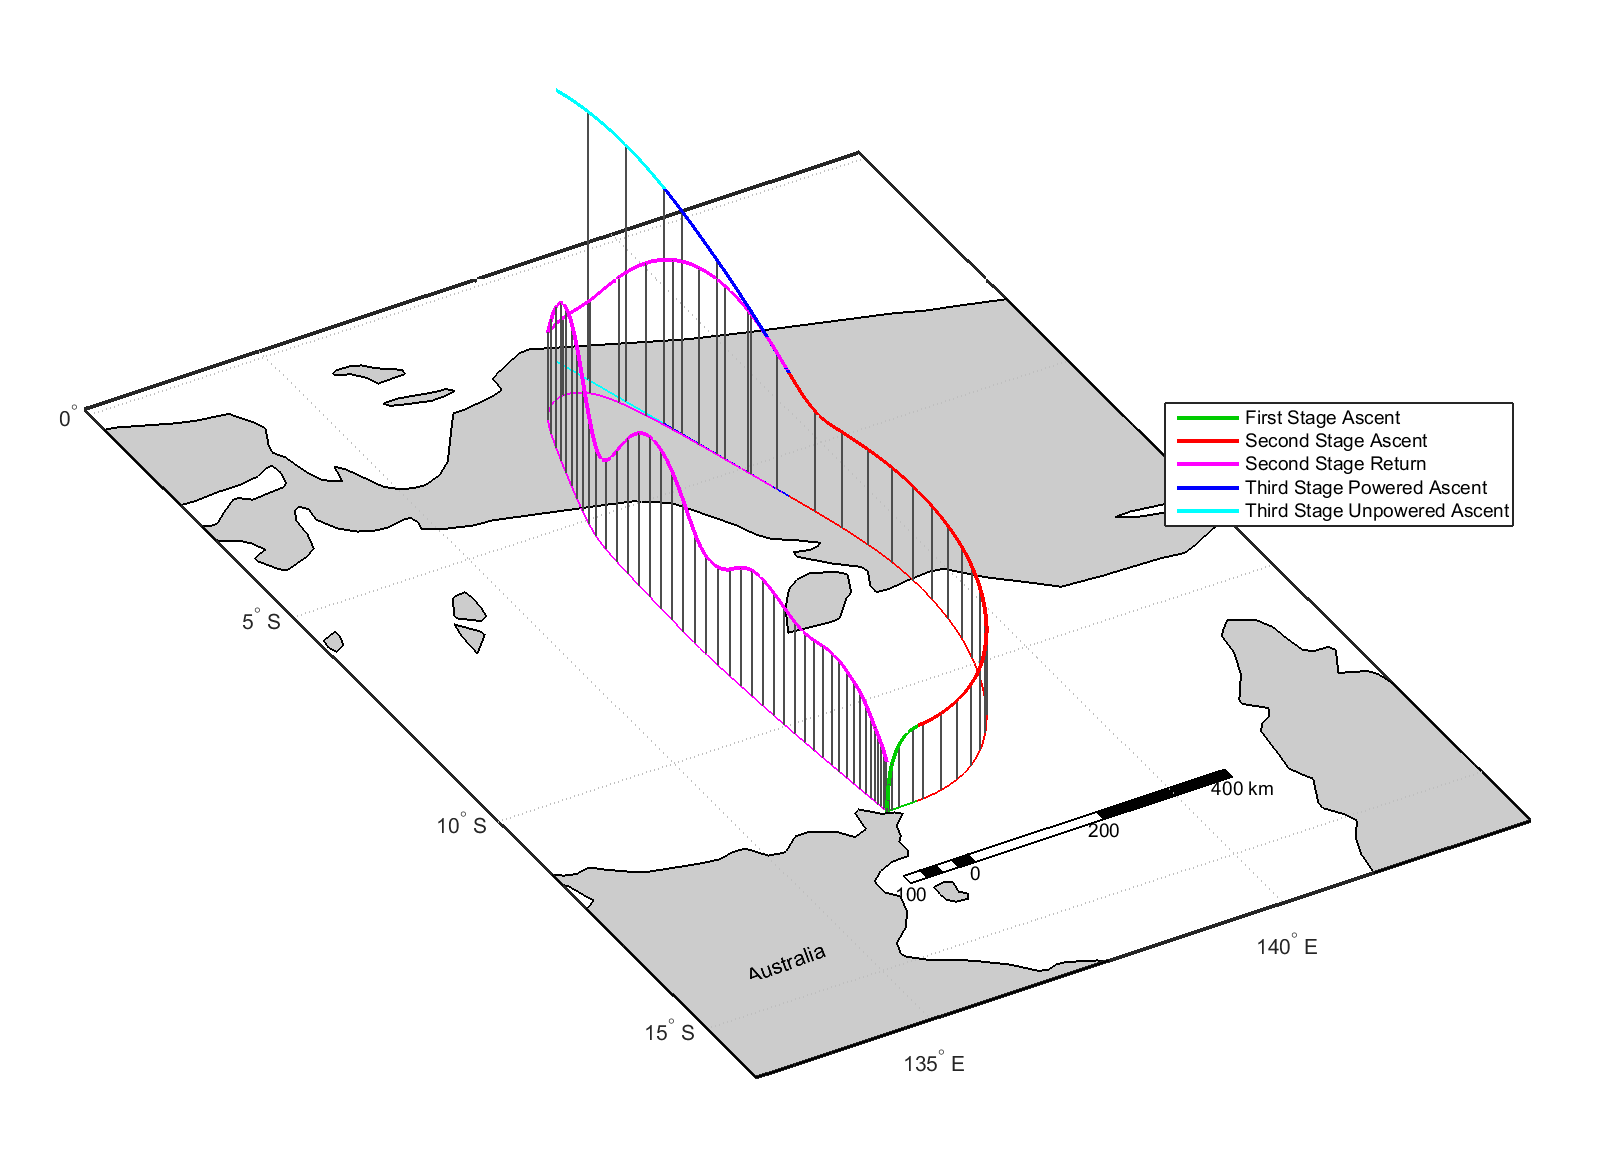
\includegraphics[width=1\linewidth]{../LODESTAR_FINAL/Results/mode10/GroundTrackStandard}
	\caption{The optimised maximum payload-to-orbit trajectory of the launch system (Case 2).}
	\label{fig:GroundTrackStandardNoReturn}
\end{figure}


The first stage trajectory, shown in Figure \ref{fig:FirstStageStandardNoReturn}, has a very similar trajectory shape to that of the first stage releasing the SPARTAN onto a constant dynamic pressure trajectory.
\begin{figure}[ht!]
	\centering
	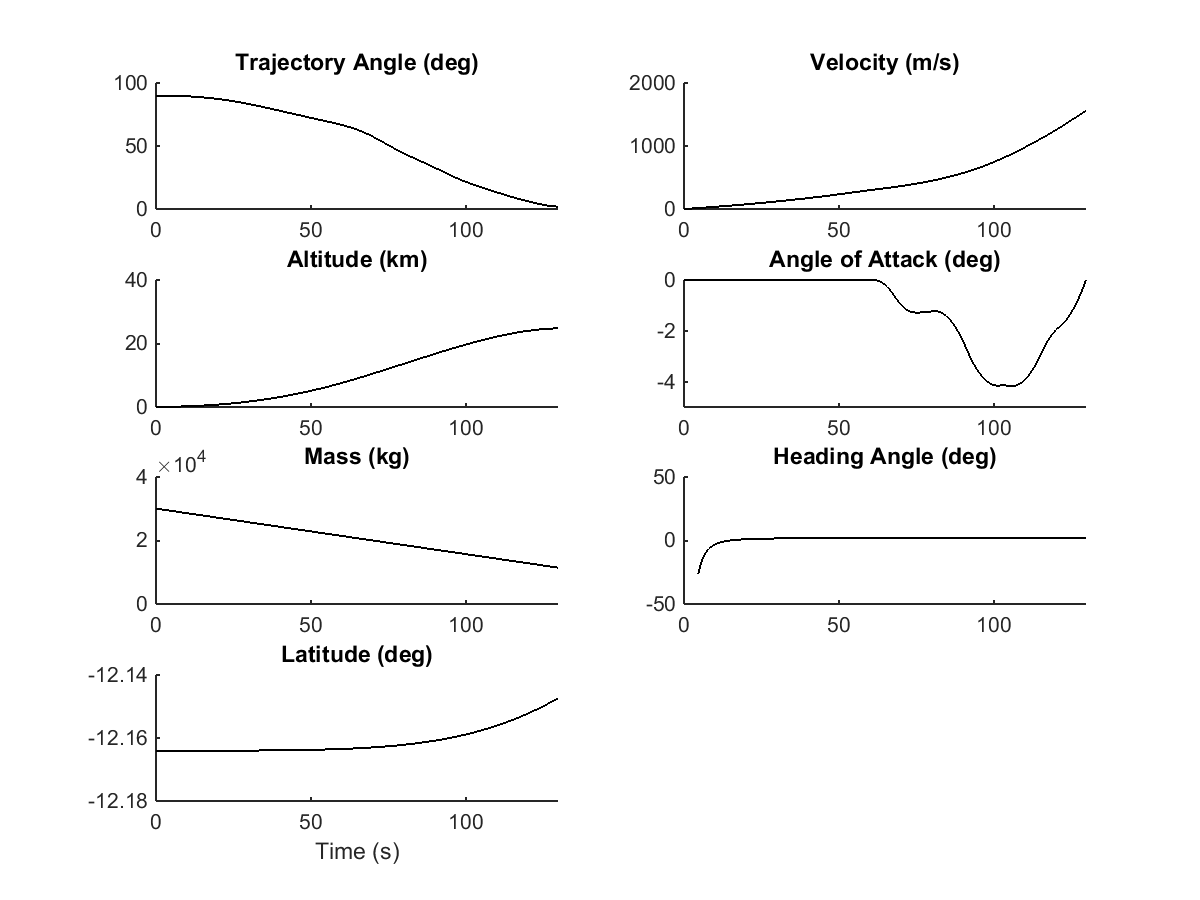
\includegraphics[width=0.9\linewidth]{../LODESTAR_FINAL/Results/mode10/FirstStageStandard}
	\caption{The optimised maximum payload-to-orbit trajectory of the launch system under power of the first stage rocket (Case 2).}
	\label{fig:FirstStageStandardNoReturn}
\end{figure}
 However, the trajectory angle at the separation of the SPARTAN is \secondthirdSeparationgammaqStandardNoReturn$^\circ$, rather than the trajectory angle of \secondthirdSeparationgammaConstq$^\circ$ required for the SPARTAN to fly a constant dynamic pressure trajectory. This higher release angle causes the altitude of the SPARTAN to immediately increase, and consequently for its dynamic pressure to decrease. This trajectory angle at release is the consequence of a trade-off between the efficiency of the SPARTAN and the first stage efficiency. The efficiency of the first stage is increased to 8.171\%, an overall improvement of 0.161\% compared to the first stage separating the SPARTAN at 50kPa conditions. 
 
 In addition to improving the exergy efficiency of the first stage, the higher release angle and altitude conditions also allow the first stage to launch with more fuel. In order to release the SPARTAN at a trajectory angle conducive to flying at 50kPa, the first stage must launch with a low fuel mass, to allow it to pitch in the correct manner. When the SPARTAN release angle and altitude are increased during the maximum payload-to-orbit trajectory, the first stage is able to launch with a fuel mass of 17185kg, an increase of 1.0\% compared to the constant dynamic pressure trajectory in Case 1. During the maximum payload-to-orbit trajectory, the first stage rocket releases the SPARTAN at a velocity of 1484.3m/s, an increase of 2.7\% compared to the first stage releasing the SPARTAN onto a constant dynamic pressure trajectory. Neither first stage utilises the full amount of allowable fuel mass, 17934kg, indicating that using the full fuel mass would necessitate separation conditions which would reduce the efficiency of the SPARTAN unfavourably. 
These results indicate that the fuel mass utilised by the first stage has a distinct optimal magnitude, and that including additional fuel over a certain amount may not increase the performance of the system. This implies that the size of the first stage is closely linked to the optimal trajectory of the system, and that future first stage designs should be sized so that optimal pitching is achieved. 

\begin{table}[ht]
	\centering
\begin{tabular}{l c } 
	\hline \textbf{Trajectory Condition}
	& StandardNoReturn

	\\
	\hline \textbf{Payload to Orbit (kg)}
	& \textbf{\PayloadToOrbitStandardNoReturn}
	\\
	\textbf{Total $\eta_{exergy}$ (\%)}
	& \textbf{\totalExergyEffStandardNoReturn}
	\\
	\hline 
	\textbf{1$^{st}$ Stage $\eta_{exergy}$ (\%)}
	& \textbf{\firstExergyEffStandardNoReturn}
	\\
	\textbf{Separation Alt, 1$\rightarrow$2 (km)}
	& \firstsecondSeparationAltStandardNoReturn
	\\
	\textbf{Separation v, 1$\rightarrow$2 (m/s)}
	& \firstsecondSeparationvStandardNoReturn
	\\
	\textbf{Separation $\gamma$, 1$\rightarrow$2 (m/s)}
	& \firstsecondSeparationgammaStandardNoReturn
	\\
	\hline 
	\textbf{2$^{nd}$ Stage $\eta_{exergy}$ (\%)}
	& \textbf{\secondExergyEffStandardNoReturn}
	\\
	\textbf{Separation Alt, 2$\rightarrow$3 (km)}
	& \secondthirdSeparationAltStandardNoReturn
	\\
	\textbf{Separation $v$, 2$\rightarrow$3 (m/s)}
	& \secondthirdSeparationvStandardNoReturn
	\\
	\textbf{Separation $\gamma$, 2$\rightarrow$3 (deg)}
	& \secondthirdSeparationgammaStandardNoReturn
	\\
	\textbf{Separation $q$, 2$\rightarrow$3(kPa)}
	& \secondthirdSeparationqStandardNoReturn
	\\
	\textbf{2$^{nd}$ Stage L/D, 2$\rightarrow$3}
	& \secondthirdSeparationLDStandardNoReturn
	\\
	\textbf{2$^{nd}$ Stage Flight Time (s)}
	& \secondFlightTimeStandardNoReturn
	\\
	\hline 
	\textbf{3$^{rd}$ Stage $\eta_{exergy}$ (\%)}
	& \textbf{\thirddExergyEffStandardNoReturn}
	\\
	\textbf{3$^{rd}$ Stage $t$, $q >$ 5kpa (s)}
	& \thirdqOverFiveStandardNoReturn
	\\
	\textbf{3$^{rd}$ Stage max $\alpha$ (deg)}
	& \thirdmaxAoAStandardNoReturn
	\\
	\textbf{3$^{rd}$ Stage Fuel Mass (kg)}
	& \thirdmFuelStandardNoReturn
	\\
	\hline 
\end{tabular} 
	\caption{A summary of key results from the maximum payload-to-orbit trajectory (Case 2).}
	\label{tab:summaryStandardNoReturn}
\end{table}







\begin{figure}[ht!]
\centering
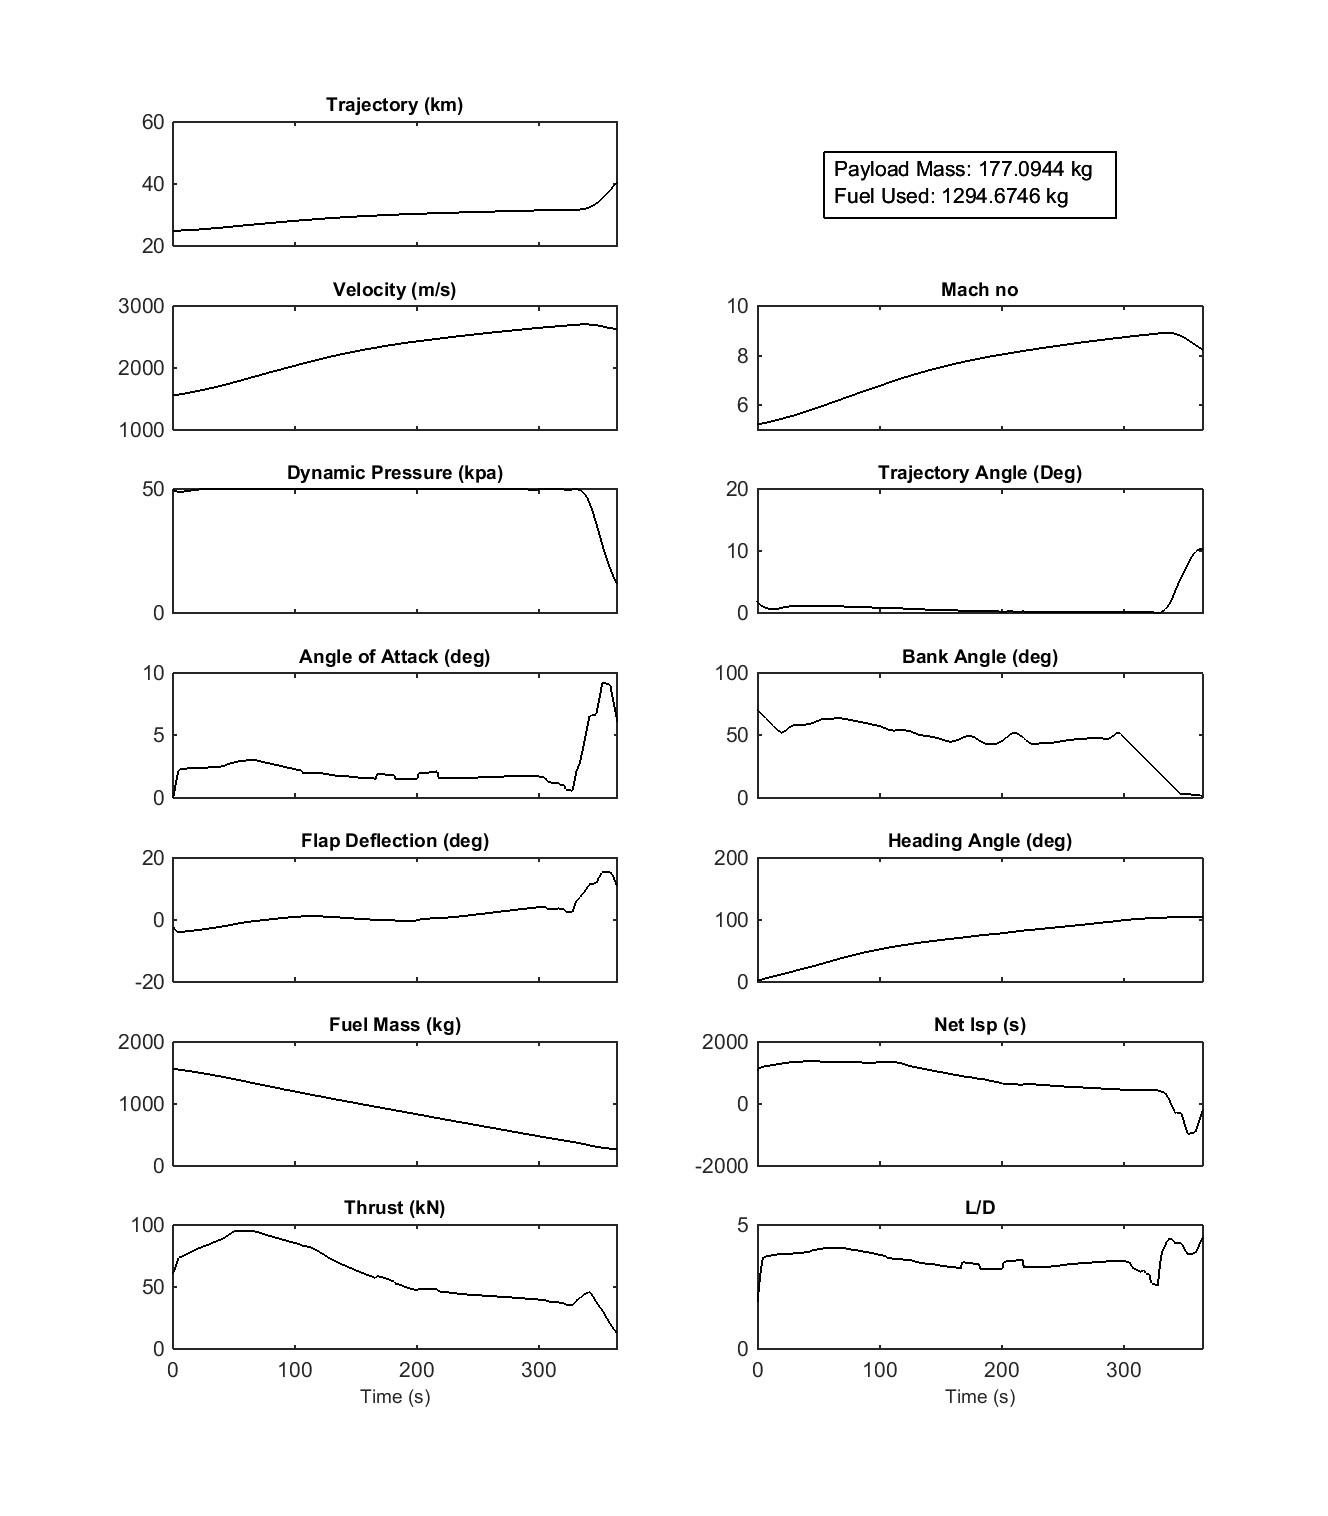
\includegraphics[width=0.9\linewidth]{../LODESTAR_FINAL/Results/mode10/SecondStageStandard}
\caption{The optimised maximum payload-to-orbit of the SPARTAN (Case 2).}
\label{fig:SecondStageStandardNoReturn}
\end{figure}



After the initial deviation from the maximum dynamic pressure, the SPARTAN returns to 50kPa dynamic pressure for a time. 
At 122.5 seconds, the altitude of the trajectory is again raised, and the dynamic pressure decreased, to a minimum of 35.6kPa. In this region the net specific impulse of the SPARTAN is relatively homogeneous with respect to changes in dynamic pressure. This homogeneous region can be observed in the specific impulse of the C-REST engines in Figure \ref{fig:IspStandard}, between inlet Mach number (M1) values of 6 and 7, and in Figure \ref{fig:NetIspStandardNoReturn}, in the Mach 7 and 8 plots of net specific impulse. This homogeneity means that the variation in engine performance with flight conditions is small and that flying at the maximum dynamic pressure in this region does not maximise the specific impulse from the C-REST engines. Figure \ref{fig:NetIspStandardNoReturn} shows that while the optimised trajectory differs significantly from a constant dynamic pressure trajectory, both achieve similar net specific impulses, with the exception of the initial trajectory conditions at Mach 5, where the efficiency of the SPARTAN is traded for first stage rocket performance. 


Appendix \ref{sec:Appendix_qconst} details a maximum payload-to-orbit trajectory in which the trajectory is constrained to 50kPa between Mach 6-8, to prevent the altitude raising manoeuvre from taking place, for comparison. 
The altitude raising manoeuvre
increases the combined total efficiency launch system from \totalExergyEffqconstrained \% to \totalExergyEffStandardNoReturn \% (calculated including stage separations). This is a relatively minor variation, and the payload-to-orbit benefits of this altitude raising manoeuvre are correspondingly small. 
The optimised trajectory exhibits a payload-to-orbit increase of 0.4kg compared to the trajectory constrained to 50kPa between Mach 6-8, a difference of only 0.2\%.
However, it is important to note that, while its benefits are small, the altitude raising manoeuvre is consistently observed in every maximum payload-to-orbit optimised trajectory. 
Also, though its benefits to payload-to-orbit are small, this altitude raising manoeuvre is significant as it reduces the heating and structural loading on the SPARTAN, though it is beyond the scope of this study to quantify these benefits. 




\begin{figure}[ht!]
	\centering
	\includegraphics[width=0.8\linewidth]{../LODESTAR_FINAL/Results/mode10/NetIspStandard}
	\caption{Net Isp contours for the SPARTAN at Mach numbers from 5-9, showing optimised trajectory and constant dynamic pressure trajectory.}
	\label{fig:NetIspStandardNoReturn}
\end{figure}

\begin{figure}[ht!]
	\centering
	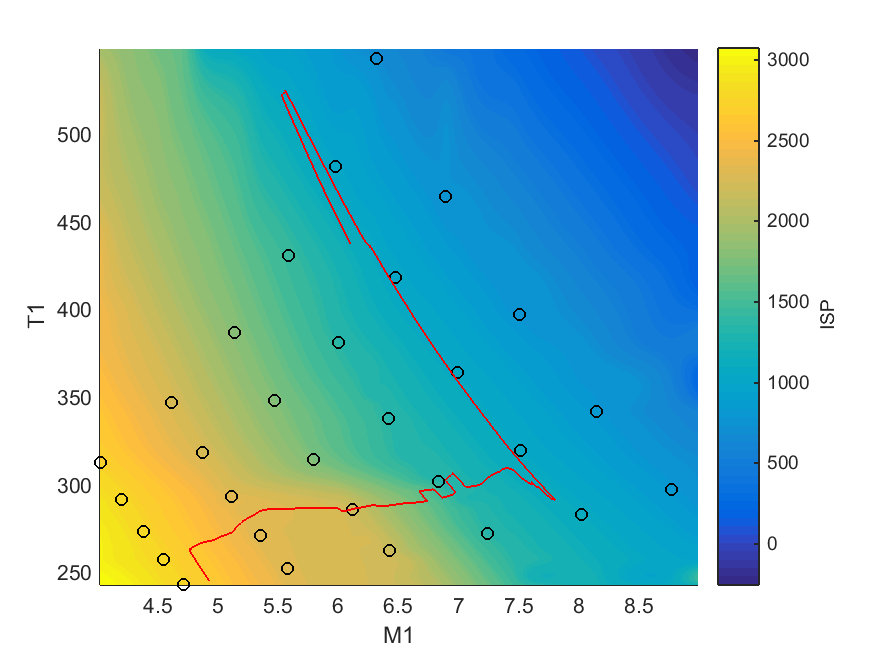
\includegraphics[width=0.8\linewidth]{../LODESTAR_FINAL/Results/mode10/IspStandard}
	\caption{The specific impulse of the C-REST engines, plotted for inlet temperature (T1) and inlet Mach number (M1). Data points are shown in black.}
	\label{fig:IspStandard}
\end{figure}


At 314.3s, the SPARTAN returns to flight at close to 50kPa dynamic pressure until 494.1s at which point a pull-up manoeuvre is performed, gaining altitude until the third stage rocket is released at 528.4s SPARTAN flight time. 
 The point at which the pull-up manoeuvre begins is the optimisation result that takes into account the best combination of velocity, altitude and release angle for scramjet stage performance and the release of the rocket stage. This pull-up indicates the region at which increasing altitude and release angle becomes more important than extracting maximum thrust from the scramjet (which is generally attained at high $q$ and low flight angle at an equivalence ratio of 1).
At high Mach numbers, flight in a lower dynamic pressure environment results in less thrust output from the scramjet engines, as well as an increase in angle of attack and flap deflection angle to compensate for the additional lift required. Due to this, less overall acceleration is obtained compared to the constant dynamic pressure result with minimum pull-up. Separation occurs at a velocity of \secondthirdSeparationvStandardNoReturn m/s, a decrease of 116.2m/s. However, at the same time separation altitude increases by 9.48km to \secondthirdSeparationAltqStandardNoReturn km, resulting in a decrease in separation dynamic pressure to \secondthirdSeparationqStandardNoReturn kPa. 
\begin{figure}[ht!]
	\centering
	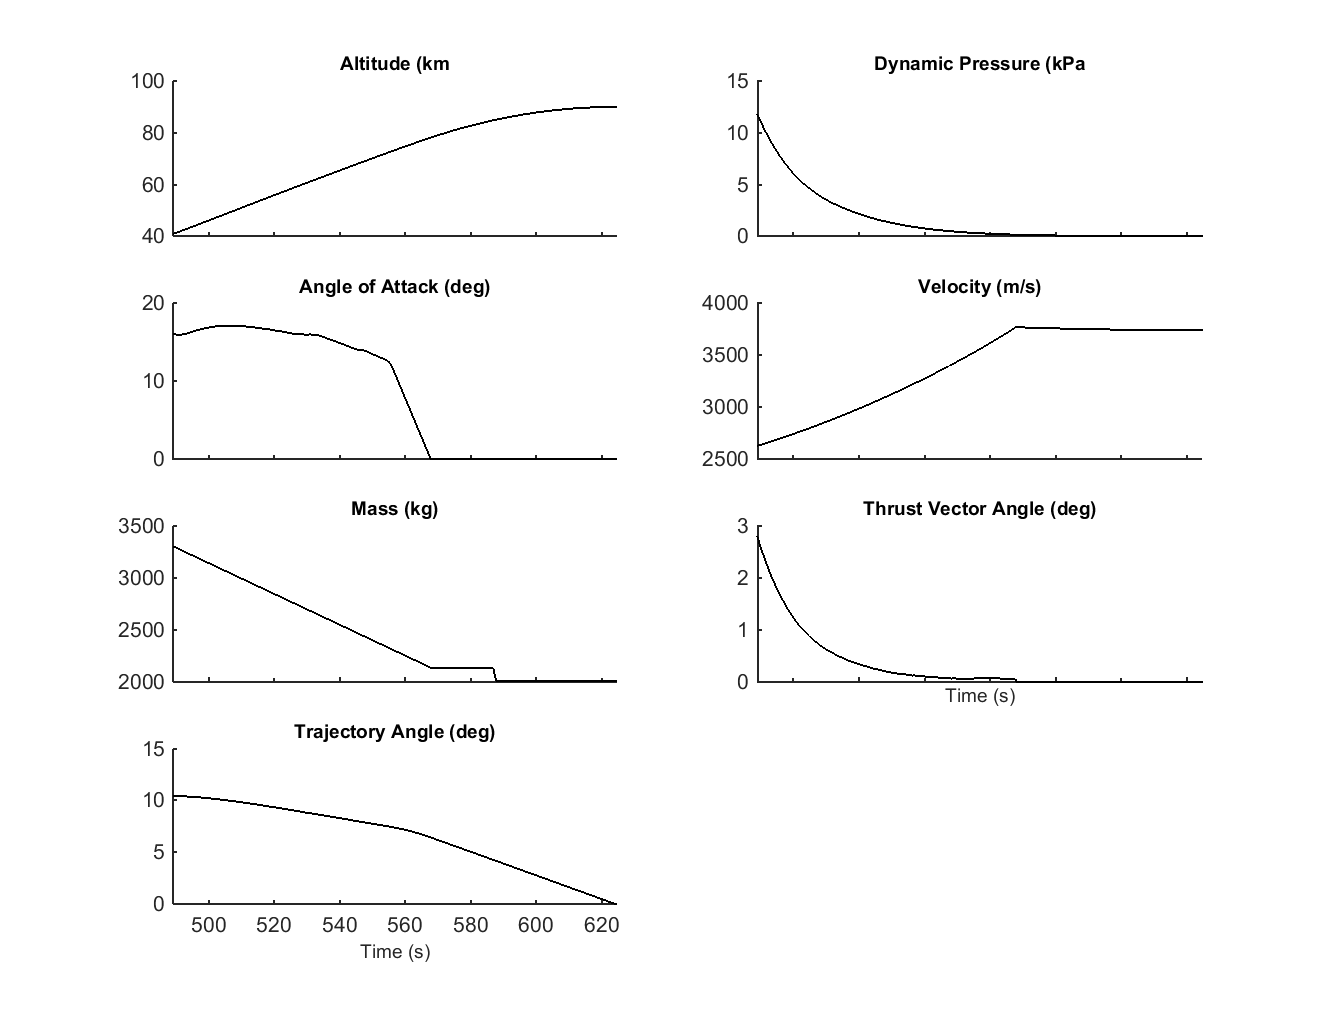
\includegraphics[width=0.9\linewidth]{../LODESTAR_FINAL/Results/mode10/ThirdStageStandard}
	\caption{The third stage trajectory of the launch system flying the maximum payload-to-orbit trajectory (Case 2).}
	\label{fig:ThirdStageStandardNoReturn}
\end{figure}
The larger scramjet stage pull-up assists the rocket in manoeuvring to exoatmospheric altitude by increasing the altitude and angle at separation by utilising the increased L/D ratio and manoeuvrability of the scramjet vehicle. The increase in release angle, to the optimal angle of \secondthirdSeparationgammaStandardNoReturn$^\circ$, significantly reduces the turning that is required by the rocket as evident from comparing Fig \ref{fig:ThirdStageConstq} and \ref{fig:ThirdStageStandardNoReturn}. 
Overall, the altitude raising manoeuvres which the SPARTAN performs result in a decrease in the exergy efficiency of the SPARTAN to \secondExergyEffStandardNoReturn \%, a total decrease of 1.318\% compared to the SPARTAN flying at a constant dynamic pressure. However, the optimised trajectory drastically increases the exergy efficiency of the third stage, to \thirddExergyEffStandardNoReturn \%, an overall increase of 6.72 \% compared to the third stage released from the SPARTAN flying a constant dynamic pressure trajectory, so that the third stage is utilising its available energy 1.61 times as efficiently.  
This leads to the total exergy efficiency of the launch system increasing from \totalExergyEffConstq \% to \totalExergyEffStandardNoReturn \%. 

The trajectory of the third stage rocket after release from an optimised scramjet trajectory is shown in Figure \ref{fig:ThirdStageStandardNoReturn}. Release at a higher, more optimal angle reduces the aerodynamic moment, in turn reducing the necessary thrust vector angle so that the thrust vector limit is not reached. The third stage rocket is released at a high trajectory angle, and continuously gains altitude, avoiding the close-to-horizontal flight required by the fixed dynamic pressure release (Case 1).
Due to the higher altitude and release angle, the third stage rocket is released at a lower dynamic pressure, \secondthirdSeparationqCdStandardNoReturn kPa compared to \secondthirdSeparationqConstq kPa, and spends much less time flying in a high dynamic pressure environment, \thirdqOverFiveStandard s at over 5kPa dynamic pressure rather than \thirdqOverFiveConstq s. 
The reduced time that the rocket must spend in a high dynamic pressure environment and decrease in the maximum dynamic pressure that the rocket stage experiences may allow the structural mass and heat shielding necessary to achieve exoatmospheric flight to be decreased. This may enable higher payload to orbit, though it is beyond the scope of this study to investigate these design changes. 


Compared to studies considering vehicles with a scramjet-rocket transition within a single stage\cite{Lu1993,Trefny1999}[CITEXX], the maximum payload to orbit trajectory of the multi-stage system shows a scramjet-rocket transition point at much lower altitudes.
This lower transition point is a consequence of the stage separation creating an energy trade-off, which does not occur in a single stage vehicle. Single-stage vehicles must necessarily transport all components to exoatmosphere, and so utilise the scramjet engines until higher altitude to take advantage of their high efficiency. A multi-stage vehicle is able to separate the scramjet stage. 
This separation occurs when the performance benefits provided by the superior aerodynamics and engine efficiency of the scramjet stage are offset by the energy required to lift the extra mass to higher altitude. The beneficial ability
to separate the scramjet stage results in a lower altitude scramjet-rocket transition point, when compared to single
stage vehicle designs.



\section{Sensitivity Analysis}\label{sec:sensitivityNoReturn}


A sensitivity analysis is conducted, in which selected design parameters of the launch system are varied, and the effects on the optimised maximum payload-to-orbit trajectory of the launch system are investigated. Appendix \ref{sec:Appendix_trajectorycomparisons} shows comparison plots of the second and third stage trajectories for each parameter variation study, however, the first stage rocket trajectories are very similar and are not shown graphically. Key results including performance factors of each stage and separation conditions are summarised within this section.
This study is performed in order to determine the relative importance of the design parameters on the efficiency of the system, as well as investigating how the maximum payload-to-orbit trajectory changes as the performance of the launch system is varied. The investigation of the key design parameters of the launch system provides a metric which can be used to quantify the relative impact of vehicle design parameters. Likewise, the optimal trajectory variation can be used to investigate the performance trade-offs between the stages. 
The information obtained from this study can be used to inform future launch system designs. 
For some of the trajectory simulations within this section, it is assumed that the scramjet engines are operable at velocities slightly under Mach 5, in order to allow meaningful assessment of parameters which effect the first stage-SPARTAN separation velocity without modification of the first stage rocket.





\textcolor{red}{I need to explain /\% better}

\textcolor{red}{state that all cases use all of the fuel available to the SPARTAN}

\subsection{Case 3: Dynamic Pressure Sensitivity}\label{sec:qvariation}

To investigate the sensitivity of the vehicle to changes in $q_{max}$, the maximum dynamic pressure is varied by $\pm$10kPa in 5kPa increments, and the flight trajectory optimised, with results shown in Table \ref{tab:qvarnoreturn}.
The variation in maximum dynamic pressure has only a small effect on the payload mass delivered to heliocentric orbit.  Varying the maximum dynamic pressure by $\pm20\%$ causes a variation of only  +7.2kg (+3.8\%) or -7.8kg (-4.1\%) in payload to orbit.  
Separation altitudes of \secondthirdSeparationAltqFortyNoReturn km and \secondthirdSeparationAltqSixtyNoReturn km are reached for the 40kPa and 60kPa limited cases respectively, with separation velocities of \secondthirdSeparationvqFortyNoReturn m/s and \secondthirdSeparationvqSixtyNoReturn m/s. The 40kPa limited case flies for \secondFlightTimeqFortyNoReturn s, significantly longer than the 60kPa case which flies for \secondFlightTimeqSixtyNoReturn s.
As the dynamic pressure decreases, the size of the altitude raising manoeuvre in the middle of the trajectory lessens. This is due to the increased altitude and angle of attack moving the flight conditions into a region where the specific impulse of the C-REST engines is not homogeneous, so that it is beneficial to fly at maximum dynamic pressure.  
All trajectories pull-up to similar altitudes, with relatively small variation in separation velocity.
This small variation in velocity is despite the increase in air density and decrease in angle of attack required for flight at higher dynamic pressures, both of which increase the mass flow into the engine. Although the thrust output of the REST engines increases with dynamic pressure, so does the drag on the vehicle, and the net increase in performance is small. 


\begin{table}[ht]
	\centering
\begin{tabular}{l c c c c c c} 
	\hline \textbf{Trajectory Condition}
	&q40
	&q45
	&q
	&q55
	&q60
	& /\%
	\\
	\hline \textbf{Payload to Orbit (kg)}
	& \textbf{\PayloadToOrbitqFortyNoReturn}
	& \textbf{\PayloadToOrbitqFortyFiveNoReturn}
	& \textbf{\PayloadToOrbitqStandardNoReturn}
	& \textbf{\PayloadToOrbitqFiftyFiveNoReturn}
	& \textbf{\PayloadToOrbitqSixtyNoReturn}
	&\textbf{0.4}
	\\
	\textbf{Payload Variation (\%)}
	& \PayloadVarqFortyNoReturn
	& \PayloadVarqFortyFiveNoReturn
	& \PayloadVarqStandardNoReturn
	& \PayloadVarqFiftyFiveNoReturn
	& \PayloadVarqSixtyNoReturn
	&0.2
	\\
	\textbf{Total $\eta_{exergy}$ (\%)}
	& \textbf{\totalExergyEffqFortyNoReturn}
	& \textbf{\totalExergyEffqFortyFiveNoReturn}
	& \textbf{\totalExergyEffqStandardNoReturn}
	& \textbf{\totalExergyEffqFiftyFiveNoReturn}
	& \textbf{\totalExergyEffqSixtyNoReturn}
	& \textbf{3e-05}
	\\
	\hline 
	\textbf{1$^{st}$ Stage $\eta_{exergy}$ (\%)}
	& \textbf{\firstExergyEffqFortyNoReturn}
	& \textbf{\firstExergyEffqFortyFiveNoReturn}
	& \textbf{\firstExergyEffqStandardNoReturn}
	& \textbf{\firstExergyEffqFiftyFiveNoReturn}
	& \textbf{\firstExergyEffqSixtyNoReturn}
	& \textbf{-0.003}
	\\
	\textbf{Separation Alt, 1$\rightarrow$2 (km)}
	& \firstsecondSeparationAltqFortyNoReturn
	& \firstsecondSeparationAltqFortyFiveNoReturn
	& \firstsecondSeparationAltqStandardNoReturn
	& \firstsecondSeparationAltqFiftyFiveNoReturn
	& \firstsecondSeparationAltqSixtyNoReturn
	&-0.06
	\\
	\textbf{Separation v, 1$\rightarrow$2 (m/s)}
	& \firstsecondSeparationvqFortyNoReturn
	& \firstsecondSeparationvqFortyFiveNoReturn
	& \firstsecondSeparationvqStandardNoReturn
	& \firstsecondSeparationvqFiftyFiveNoReturn
	& \firstsecondSeparationvqSixtyNoReturn
	& -
	\\
	\textbf{Separation $\gamma$, 1$\rightarrow$2 (m/s)}
	& \firstsecondSeparationgammaqFortyNoReturn
	& \firstsecondSeparationgammaqFortyFiveNoReturn
	& \firstsecondSeparationgammaqStandardNoReturn
	& \firstsecondSeparationgammaqFiftyFiveNoReturn
	& \firstsecondSeparationgammaqSixtyNoReturn
	&-0.13
	\\
	\hline 
	\textbf{2$^{nd}$ Stage $\eta_{exergy}$ (\%)}
	& \textbf{\secondExergyEffqFortyNoReturn}
	& \textbf{\secondExergyEffqFortyFiveNoReturn}
	& \textbf{\secondExergyEffqStandardNoReturn}
	& \textbf{\secondExergyEffqFiftyFiveNoReturn}
	& \textbf{\secondExergyEffqSixtyNoReturn}
	& \textbf{0.02}
	\\
	\textbf{Separation Alt, 2$\rightarrow$3 (km)}
	& \secondthirdSeparationAltqFortyNoReturn
	& \secondthirdSeparationAltqFortyFiveNoReturn
	& \secondthirdSeparationAltqStandardNoReturn
	& \secondthirdSeparationAltqFiftyFiveNoReturn
	& \secondthirdSeparationAltqSixtyNoReturn
	&-0.02
	\\
	\textbf{Separation $v$, 2$\rightarrow$3 (m/s)}
	& \secondthirdSeparationvqFortyNoReturn
	& \secondthirdSeparationvqFortyFiveNoReturn
	& \secondthirdSeparationvqStandardNoReturn
	& \secondthirdSeparationvqFiftyFiveNoReturn
	& \secondthirdSeparationvqSixtyNoReturn
	&1.56
	\\
	\textbf{Separation $\gamma$, 2$\rightarrow$3 (deg)}
	& \secondthirdSeparationgammaqFortyNoReturn
	& \secondthirdSeparationgammaqFortyFiveNoReturn
	& \secondthirdSeparationgammaqStandardNoReturn
	& \secondthirdSeparationgammaqFiftyFiveNoReturn
	& \secondthirdSeparationgammaqSixtyNoReturn
	&0.03
	\\
	\textbf{Separation $q$, 2$\rightarrow$3(kPa)}
	& \secondthirdSeparationqqFortyNoReturn
	& \secondthirdSeparationqqFortyFiveNoReturn
	& \secondthirdSeparationqqStandardNoReturn
	& \secondthirdSeparationqqFiftyFiveNoReturn
	& \secondthirdSeparationqqSixtyNoReturn
	&0.04
	\\
	\textbf{2$^{nd}$ Stage L/D, 2$\rightarrow$3}
	& \secondthirdSeparationLDqFortyNoReturn
	& \secondthirdSeparationLDqFortyFiveNoReturn
	& \secondthirdSeparationLDqStandardNoReturn
	& \secondthirdSeparationLDqFiftyFiveNoReturn
	& \secondthirdSeparationLDqSixtyNoReturn
	& -
	\\
	\textbf{2$^{nd}$ Stage Flight Time (s)}
	& \secondFlightTimeqFortyNoReturn
	& \secondFlightTimeqFortyFiveNoReturn
	& \secondFlightTimeqStandardNoReturn
	& \secondFlightTimeqFiftyFiveNoReturn
	& \secondFlightTimeqSixtyNoReturn
	&-3.62
	\\
	\hline 
	\textbf{3$^{rd}$ Stage $\eta_{exergy}$ (\%)}
	& \textbf{\thirddExergyEffqFortyNoReturn}
	& \textbf{\thirddExergyEffqFortyFiveNoReturn}
	& \textbf{\thirddExergyEffqStandardNoReturn}
	& \textbf{\thirddExergyEffqFiftyFiveNoReturn}
	& \textbf{\thirddExergyEffqSixtyNoReturn}
	& -
	\\
	\textbf{3$^{rd}$ Stage $t$, $q >$ 5kpa (s)}
	& \thirdqOverFiveqFortyNoReturn
	& \thirdqOverFiveqFortyFiveNoReturn
	& \thirdqOverFiveqStandardNoReturn
	& \thirdqOverFiveqFiftyFiveNoReturn
	& \thirdqOverFiveqSixtyNoReturn
	& -
	\\
	\textbf{3$^{rd}$ Stage max $\alpha$ (deg)}
	& \thirdmaxAoAqFortyNoReturn
	& \thirdmaxAoAqFortyFiveNoReturn
	& \thirdmaxAoAqStandardNoReturn
	& \thirdmaxAoAqFiftyFiveNoReturn
	& \thirdmaxAoAqSixtyNoReturn
	&0
	\\
	\textbf{3$^{rd}$ Stage Fuel Mass (kg)}
	& \thirdmFuelqFortyNoReturn
	& \thirdmFuelqFortyFiveNoReturn
	& \thirdmFuelqStandardNoReturn
	& \thirdmFuelqFiftyFiveNoReturn
	& \thirdmFuelqSixtyNoReturn
	&-0.37
	\\
	\hline 
\end{tabular} 
 \caption{}
 \label{tab:qvarnoreturn}
\end{table}

Only a small variation in optimal payload mass is observed, without modification of vehicle design to account for the dynamic pressure limit. This indicates that designing and operating a vehicle at lower dynamic pressures may be preferable. Flying at a lower maximum dynamic pressure allows reduction of the structural weight and heat shielding of the vehicle[CITEXX?]. 
While it is outside the scope of this study to directly estimate the thermal shielding mass increase necessary when increasing the maximum allowable dynamic pressure, it can be observed from Section \ref{sec:SpartanMassnoreturn} that the influence of the SPARTAN's mass on the performance of the system is large. The decrease in thermal protection system mass possible for lower dynamic pressure trajectories, which is likely to be significant, will serve to partially offset the minor loss in payload due to lower dynamic pressure operation. 
\textcolor{red}{need to directly compare with mass variation study, to estimate magnitude of thermal mass variation which will make flying at lower q valuable}



\subsection{Case 4: SPARTAN Drag Sensitivity}\label{sec:dragvariation}

\begin{table}[ht!]
	\centering
	\begin{tabular}{l c c c c c c} 
		\hline \textbf{Trajectory Condition}
		&Cd90
		&Cd95
		&Cd
		&Cd105
		&Cd110
		& /\%
		\\
		\hline \textbf{Payload to Orbit (kg)}
		& \textbf{\PayloadToOrbitCdNinetyNoReturn}
		& \textbf{\PayloadToOrbitCdNinetyFiveNoReturn}
		& \textbf{\PayloadToOrbitCdStandardNoReturn}
		& \textbf{\PayloadToOrbitCdOneHundredFiveNoReturn}
		& \textbf{\PayloadToOrbitCdOneHundredTenNoReturn}
		&\textbf{-1.9}
		\\
		\textbf{Payload Variation (\%)}
		& \PayloadVarCdNinetyNoReturn
		& \PayloadVarCdNinetyFiveNoReturn
		& \PayloadVarCdStandardNoReturn
		& \PayloadVarCdOneHundredFiveNoReturn
		& \PayloadVarCdOneHundredTenNoReturn
		&-0.99
		\\
		\textbf{Total $\eta_{exergy}$ (\%)}
		& \textbf{\totalExergyEffCdNinetyNoReturn}
		& \textbf{\totalExergyEffCdNinetyFiveNoReturn}
		& \textbf{\totalExergyEffCdStandardNoReturn}
		& \textbf{\totalExergyEffCdOneHundredFiveNoReturn}
		& \textbf{\totalExergyEffCdOneHundredTenNoReturn}
		& \textbf{-0.00016}
		\\
		\hline 
		\textbf{1$^{st}$ Stage $\eta_{exergy}$ (\%)}
		& \textbf{\firstExergyEffCdNinetyNoReturn}
		& \textbf{\firstExergyEffCdNinetyFiveNoReturn}
		& \textbf{\firstExergyEffCdStandardNoReturn}
		& \textbf{\firstExergyEffCdOneHundredFiveNoReturn}
		& \textbf{\firstExergyEffCdOneHundredTenNoReturn}
		& \textbf{-0.041}
		\\
		\textbf{Separation Alt, 1$\rightarrow$2 (km)}
		& \firstsecondSeparationAltCdNinetyNoReturn
		& \firstsecondSeparationAltCdNinetyFiveNoReturn
		& \firstsecondSeparationAltCdStandardNoReturn
		& \firstsecondSeparationAltCdOneHundredFiveNoReturn
		& \firstsecondSeparationAltCdOneHundredTenNoReturn
		&-0.09
		\\
		\textbf{Separation v, 1$\rightarrow$2 (m/s)}
		& \firstsecondSeparationvCdNinetyNoReturn
		& \firstsecondSeparationvCdNinetyFiveNoReturn
		& \firstsecondSeparationvCdStandardNoReturn
		& \firstsecondSeparationvCdOneHundredFiveNoReturn
		& \firstsecondSeparationvCdOneHundredTenNoReturn
		&-4.87
		\\
		\textbf{Separation $\gamma$, 1$\rightarrow$2 (m/s)}
		& \firstsecondSeparationgammaCdNinetyNoReturn
		& \firstsecondSeparationgammaCdNinetyFiveNoReturn
		& \firstsecondSeparationgammaCdStandardNoReturn
		& \firstsecondSeparationgammaCdOneHundredFiveNoReturn
		& \firstsecondSeparationgammaCdOneHundredTenNoReturn
		&-0.22
		\\
		\hline 
		\textbf{2$^{nd}$ Stage $\eta_{exergy}$ (\%)}
		& \textbf{\secondExergyEffCdNinetyNoReturn}
		& \textbf{\secondExergyEffCdNinetyFiveNoReturn}
		& \textbf{\secondExergyEffCdStandardNoReturn}
		& \textbf{\secondExergyEffCdOneHundredFiveNoReturn}
		& \textbf{\secondExergyEffCdOneHundredTenNoReturn}
		& \textbf{-0.086}
		\\
		\textbf{Separation Alt, 2$\rightarrow$3 (km)}
		& \secondthirdSeparationAltCdNinetyNoReturn
		& \secondthirdSeparationAltCdNinetyFiveNoReturn
		& \secondthirdSeparationAltCdStandardNoReturn
		& \secondthirdSeparationAltCdOneHundredFiveNoReturn
		& \secondthirdSeparationAltCdOneHundredTenNoReturn
		& -
		\\
		\textbf{Separation $v$, 2$\rightarrow$3 (m/s)}
		& \secondthirdSeparationvCdNinetyNoReturn
		& \secondthirdSeparationvCdNinetyFiveNoReturn
		& \secondthirdSeparationvCdStandardNoReturn
		& \secondthirdSeparationvCdOneHundredFiveNoReturn
		& \secondthirdSeparationvCdOneHundredTenNoReturn
		&-10.69
		\\
		\textbf{Separation $\gamma$, 2$\rightarrow$3 (deg)}
		& \secondthirdSeparationgammaCdNinetyNoReturn
		& \secondthirdSeparationgammaCdNinetyFiveNoReturn
		& \secondthirdSeparationgammaCdStandardNoReturn
		& \secondthirdSeparationgammaCdOneHundredFiveNoReturn
		& \secondthirdSeparationgammaCdOneHundredTenNoReturn
		& -
		\\
		\textbf{Separation $q$, 2$\rightarrow$3(kPa)}
		& \secondthirdSeparationqCdNinetyNoReturn
		& \secondthirdSeparationqCdNinetyFiveNoReturn
		& \secondthirdSeparationqCdStandardNoReturn
		& \secondthirdSeparationqCdOneHundredFiveNoReturn
		& \secondthirdSeparationqCdOneHundredTenNoReturn
		& -
		\\
		\textbf{2$^{nd}$ Stage L/D, 2$\rightarrow$3}
		& \secondthirdSeparationLDCdNinetyNoReturn
		& \secondthirdSeparationLDCdNinetyFiveNoReturn
		& \secondthirdSeparationLDCdStandardNoReturn
		& \secondthirdSeparationLDCdOneHundredFiveNoReturn
		& \secondthirdSeparationLDCdOneHundredTenNoReturn
		&-0.02
		\\
		\textbf{2$^{nd}$ Stage Flight Time (s)}
		& \secondFlightTimeCdNinetyNoReturn
		& \secondFlightTimeCdNinetyFiveNoReturn
		& \secondFlightTimeCdStandardNoReturn
		& \secondFlightTimeCdOneHundredFiveNoReturn
		& \secondFlightTimeCdOneHundredTenNoReturn
		& -
		\\
		\hline 
		\textbf{3$^{rd}$ Stage $\eta_{exergy}$ (\%)}
		& \textbf{\thirddExergyEffCdNinetyNoReturn}
		& \textbf{\thirddExergyEffCdNinetyFiveNoReturn}
		& \textbf{\thirddExergyEffCdStandardNoReturn}
		& \textbf{\thirddExergyEffCdOneHundredFiveNoReturn}
		& \textbf{\thirddExergyEffCdOneHundredTenNoReturn}
		& \textbf{0.047}
		\\
		\textbf{3$^{rd}$ Stage $t$, $q >$ 5kpa (s)}
		& \thirdqOverFiveCdNinetyNoReturn
		& \thirdqOverFiveCdNinetyFiveNoReturn
		& \thirdqOverFiveCdStandardNoReturn
		& \thirdqOverFiveCdOneHundredFiveNoReturn
		& \thirdqOverFiveCdOneHundredTenNoReturn
		& -
		\\
		\textbf{3$^{rd}$ Stage max $\alpha$ (deg)}
		& \thirdmaxAoACdNinetyNoReturn
		& \thirdmaxAoACdNinetyFiveNoReturn
		& \thirdmaxAoACdStandardNoReturn
		& \thirdmaxAoACdOneHundredFiveNoReturn
		& \thirdmaxAoACdOneHundredTenNoReturn
		& -
		\\
		\textbf{3$^{rd}$ Stage Fuel Mass (kg)}
		& \thirdmFuelCdNinetyNoReturn
		& \thirdmFuelCdNinetyFiveNoReturn
		& \thirdmFuelCdStandardNoReturn
		& \thirdmFuelCdOneHundredFiveNoReturn
		& \thirdmFuelCdOneHundredTenNoReturn
		&1.86
		\\
		\hline 
	\end{tabular} 
	\caption{}
	\label{tab:DragVariationNoReturn}
\end{table}

To investigate the effect of vehicle design and uncertainty in aerodynamic performance on the optimal trajectory the drag on the vehicle is varied by $\pm10$\%, and an optimised trajectory calculated with dynamic pressure limited to 50kpa. Results are compared to the 100\% drag result in \ref{tab:DragVariationNoReturn} with a trajectory path comparison shown in Appendix \ref{sec:Appendix_trajectorycomparisons}. 

The velocity and trajectory angle at first stage-SPARTAN separation decrease significantly as the drag is increased. This indicates that as the drag increases, the first stage accelerates more slowly, and is consequently able to pitch more during the trajectory.
The SPARTAN trajectory results show that when drag is varied, the optimal trajectories are similar to the base-line case, with a similarly sized pull-up, though as the drag is increased (ie. L/D is decreased), the second stage follows a slightly slower and hence lower flight path. The similar flight path shape of the high drag case suggests that sacrificing velocity to increase separation altitude in a pull-up manoeuvre is optimal for multiple vehicle designs, and that the size of this pull-up is consistent with variation in the aerodynamics of the SPARTAN.



\subsection{Case 5: C-REST Engine Specific Impulse Sensitivity}

\begin{table}[ht!]
	\centering
	\begin{tabular}{l c c c c c c} 
		\hline \textbf{Trajectory Condition}
		&Isp90
		&Isp95
		&Isp
		&Isp105
		&Isp110
		& /\%
		\\
		\hline \textbf{Payload to Orbit (kg)}
		& \textbf{\PayloadToOrbitIspNinetyNoReturn}
		& \textbf{\PayloadToOrbitIspNinetyFiveNoReturn}
		& \textbf{\PayloadToOrbitIspStandardNoReturn}
		& \textbf{\PayloadToOrbitIspOneHundredFiveNoReturn}
		& \textbf{\PayloadToOrbitIspOneHundredTenNoReturn}
		&\textbf{2.2}
		\\
		\textbf{Payload Variation (\%)}
		& \PayloadVarIspNinetyNoReturn
		& \PayloadVarIspNinetyFiveNoReturn
		& \PayloadVarIspStandardNoReturn
		& \PayloadVarIspOneHundredFiveNoReturn
		& \PayloadVarIspOneHundredTenNoReturn
		&1.16
		\\
		\textbf{Total $\eta_{exergy}$ (\%)}
		& \textbf{\totalExergyEffIspNinetyNoReturn}
		& \textbf{\totalExergyEffIspNinetyFiveNoReturn}
		& \textbf{\totalExergyEffIspStandardNoReturn}
		& \textbf{\totalExergyEffIspOneHundredFiveNoReturn}
		& \textbf{\totalExergyEffIspOneHundredTenNoReturn}
		& \textbf{0.0002}
		\\
		\hline 
		\textbf{1$^{st}$ Stage $\eta_{exergy}$ (\%)}
		& \textbf{\firstExergyEffIspNinetyNoReturn}
		& \textbf{\firstExergyEffIspNinetyFiveNoReturn}
		& \textbf{\firstExergyEffIspStandardNoReturn}
		& \textbf{\firstExergyEffIspOneHundredFiveNoReturn}
		& \textbf{\firstExergyEffIspOneHundredTenNoReturn}
		& -
		\\
		\textbf{Separation Alt, 1$\rightarrow$2 (km)}
		& \firstsecondSeparationAltIspNinetyNoReturn
		& \firstsecondSeparationAltIspNinetyFiveNoReturn
		& \firstsecondSeparationAltIspStandardNoReturn
		& \firstsecondSeparationAltIspOneHundredFiveNoReturn
		& \firstsecondSeparationAltIspOneHundredTenNoReturn
		& -
		\\
		\textbf{Separation v, 1$\rightarrow$2 (m/s)}
		& \firstsecondSeparationvIspNinetyNoReturn
		& \firstsecondSeparationvIspNinetyFiveNoReturn
		& \firstsecondSeparationvIspStandardNoReturn
		& \firstsecondSeparationvIspOneHundredFiveNoReturn
		& \firstsecondSeparationvIspOneHundredTenNoReturn
		& -
		\\
		\textbf{Separation $\gamma$, 1$\rightarrow$2 (m/s)}
		& \firstsecondSeparationgammaIspNinetyNoReturn
		& \firstsecondSeparationgammaIspNinetyFiveNoReturn
		& \firstsecondSeparationgammaIspStandardNoReturn
		& \firstsecondSeparationgammaIspOneHundredFiveNoReturn
		& \firstsecondSeparationgammaIspOneHundredTenNoReturn
		& -
		\\
		\hline 
		\textbf{2$^{nd}$ Stage $\eta_{exergy}$ (\%)}
		& \textbf{\secondExergyEffIspNinetyNoReturn}
		& \textbf{\secondExergyEffIspNinetyFiveNoReturn}
		& \textbf{\secondExergyEffIspStandardNoReturn}
		& \textbf{\secondExergyEffIspOneHundredFiveNoReturn}
		& \textbf{\secondExergyEffIspOneHundredTenNoReturn}
		& \textbf{0.162}
		\\
		\textbf{Separation Alt, 2$\rightarrow$3 (km)}
		& \secondthirdSeparationAltIspNinetyNoReturn
		& \secondthirdSeparationAltIspNinetyFiveNoReturn
		& \secondthirdSeparationAltIspStandardNoReturn
		& \secondthirdSeparationAltIspOneHundredFiveNoReturn
		& \secondthirdSeparationAltIspOneHundredTenNoReturn
		& -
		\\
		\textbf{Separation $v$, 2$\rightarrow$3 (m/s)}
		& \secondthirdSeparationvIspNinetyNoReturn
		& \secondthirdSeparationvIspNinetyFiveNoReturn
		& \secondthirdSeparationvIspStandardNoReturn
		& \secondthirdSeparationvIspOneHundredFiveNoReturn
		& \secondthirdSeparationvIspOneHundredTenNoReturn
		&13.74
		\\
		\textbf{Separation $\gamma$, 2$\rightarrow$3 (deg)}
		& \secondthirdSeparationgammaIspNinetyNoReturn
		& \secondthirdSeparationgammaIspNinetyFiveNoReturn
		& \secondthirdSeparationgammaIspStandardNoReturn
		& \secondthirdSeparationgammaIspOneHundredFiveNoReturn
		& \secondthirdSeparationgammaIspOneHundredTenNoReturn
		&-0.08
		\\
		\textbf{Separation $q$, 2$\rightarrow$3(kPa)}
		& \secondthirdSeparationqIspNinetyNoReturn
		& \secondthirdSeparationqIspNinetyFiveNoReturn
		& \secondthirdSeparationqIspStandardNoReturn
		& \secondthirdSeparationqIspOneHundredFiveNoReturn
		& \secondthirdSeparationqIspOneHundredTenNoReturn
		& -
		\\
		\textbf{2$^{nd}$ Stage L/D, 2$\rightarrow$3}
		& \secondthirdSeparationLDIspNinetyNoReturn
		& \secondthirdSeparationLDIspNinetyFiveNoReturn
		& \secondthirdSeparationLDIspStandardNoReturn
		& \secondthirdSeparationLDIspOneHundredFiveNoReturn
		& \secondthirdSeparationLDIspOneHundredTenNoReturn
		& -
		\\
		\textbf{2$^{nd}$ Stage Flight Time (s)}
		& \secondFlightTimeIspNinetyNoReturn
		& \secondFlightTimeIspNinetyFiveNoReturn
		& \secondFlightTimeIspStandardNoReturn
		& \secondFlightTimeIspOneHundredFiveNoReturn
		& \secondFlightTimeIspOneHundredTenNoReturn
		& -
		\\
		\hline 
		\textbf{3$^{rd}$ Stage $\eta_{exergy}$ (\%)}
		& \textbf{\thirddExergyEffIspNinetyNoReturn}
		& \textbf{\thirddExergyEffIspNinetyFiveNoReturn}
		& \textbf{\thirddExergyEffIspStandardNoReturn}
		& \textbf{\thirddExergyEffIspOneHundredFiveNoReturn}
		& \textbf{\thirddExergyEffIspOneHundredTenNoReturn}
		& \textbf{-0.073}
		\\
		\textbf{3$^{rd}$ Stage $t$, $q >$ 5kpa (s)}
		& \thirdqOverFiveIspNinetyNoReturn
		& \thirdqOverFiveIspNinetyFiveNoReturn
		& \thirdqOverFiveIspStandardNoReturn
		& \thirdqOverFiveIspOneHundredFiveNoReturn
		& \thirdqOverFiveIspOneHundredTenNoReturn
		& -
		\\
		\textbf{3$^{rd}$ Stage max $\alpha$ (deg)}
		& \thirdmaxAoAIspNinetyNoReturn
		& \thirdmaxAoAIspNinetyFiveNoReturn
		& \thirdmaxAoAIspStandardNoReturn
		& \thirdmaxAoAIspOneHundredFiveNoReturn
		& \thirdmaxAoAIspOneHundredTenNoReturn
		& -
		\\
		\textbf{3$^{rd}$ Stage Fuel Mass (kg)}
		& \thirdmFuelIspNinetyNoReturn
		& \thirdmFuelIspNinetyFiveNoReturn
		& \thirdmFuelIspStandardNoReturn
		& \thirdmFuelIspOneHundredFiveNoReturn
		& \thirdmFuelIspOneHundredTenNoReturn
		&-2.2
		\\
		\hline 
	\end{tabular} 
	
\end{table}

The specific impulse of the C-REST scramjet engines is varied by $\pm10\%$ to directly investigate the effects of the efficiency of the scramjet engines on the performance of the launch vehicle. 
The additional efficiency allows the SPARTAN to accelerate more over the flight time, increasing the velocity at SPARTAN-third stage separation significantly. The velocity added to the end of the SPARTAN's trajectory directly contributes to the final velocity of the third stage at circularisation. Varying the specific impulse does not change the optimal SPARTAN-third stage separation altitude significantly, however the increased velocity allows this altitude to be reached by the SPARTAN with less trajectory angle variation during the pull-up, and allows the third stage to successfully reach orbit from a lower trajectory angle release point.




\subsection{Case 6: SPARTAN Mass Sensitivity}\label{sec:SpartanMassnoreturn}



\begin{table}[ht]
	\centering
	
	
\begin{tabular}{l c c c c c c} 
	\hline \textbf{Trajectory Condition}
	&m295
	&m297.5
	&m2
	&m2102.5
	&m2105
	& /\%
	\\
	\hline \textbf{Payload to Orbit (kg)}
	& \textbf{\PayloadToOrbitmSPARTANNinetyFiveNoReturn}
	& \textbf{\PayloadToOrbitmSPARTANNinetySevenFiveNoReturn}
	& \textbf{\PayloadToOrbitmSPARTANStandardNoReturn}
	& \textbf{\PayloadToOrbitmSPARTANOneHundredTwoFiveNoReturn}
	& \textbf{\PayloadToOrbitmSPARTANOneHundredFiveNoReturn}
	&\textbf{-1.5}
	\\
	\textbf{Payload Variation (\%)}
	& \PayloadVarmSPARTANNinetyFiveNoReturn
	& \PayloadVarmSPARTANNinetySevenFiveNoReturn
	& \PayloadVarmSPARTANStandardNoReturn
	& \PayloadVarmSPARTANOneHundredTwoFiveNoReturn
	& \PayloadVarmSPARTANOneHundredFiveNoReturn
	&-0.8
	\\
	\textbf{Total $\eta_{exergy}$ (\%)}
	& \textbf{\totalExergyEffmSPARTANNinetyFiveNoReturn}
	& \textbf{\totalExergyEffmSPARTANNinetySevenFiveNoReturn}
	& \textbf{\totalExergyEffmSPARTANStandardNoReturn}
	& \textbf{\totalExergyEffmSPARTANOneHundredTwoFiveNoReturn}
	& \textbf{\totalExergyEffmSPARTANOneHundredFiveNoReturn}
	& \textbf{-0.00011}
	\\
	\hline 
	\textbf{1$^{st}$ Stage $\eta_{exergy}$ (\%)}
	& \textbf{\firstExergyEffmSPARTANNinetyFiveNoReturn}
	& \textbf{\firstExergyEffmSPARTANNinetySevenFiveNoReturn}
	& \textbf{\firstExergyEffmSPARTANStandardNoReturn}
	& \textbf{\firstExergyEffmSPARTANOneHundredTwoFiveNoReturn}
	& \textbf{\firstExergyEffmSPARTANOneHundredFiveNoReturn}
	& \textbf{-0.06}
	\\
	\textbf{Separation Alt, 1$\rightarrow$2 (km)}
	& \firstsecondSeparationAltmSPARTANNinetyFiveNoReturn
	& \firstsecondSeparationAltmSPARTANNinetySevenFiveNoReturn
	& \firstsecondSeparationAltmSPARTANStandardNoReturn
	& \firstsecondSeparationAltmSPARTANOneHundredTwoFiveNoReturn
	& \firstsecondSeparationAltmSPARTANOneHundredFiveNoReturn
	&-0.22
	\\
	\textbf{Separation v, 1$\rightarrow$2 (m/s)}
	& \firstsecondSeparationvmSPARTANNinetyFiveNoReturn
	& \firstsecondSeparationvmSPARTANNinetySevenFiveNoReturn
	& \firstsecondSeparationvmSPARTANStandardNoReturn
	& \firstsecondSeparationvmSPARTANOneHundredTwoFiveNoReturn
	& \firstsecondSeparationvmSPARTANOneHundredFiveNoReturn
	&-11.97
	\\
	\textbf{Separation $\gamma$, 1$\rightarrow$2 (m/s)}
	& \firstsecondSeparationgammamSPARTANNinetyFiveNoReturn
	& \firstsecondSeparationgammamSPARTANNinetySevenFiveNoReturn
	& \firstsecondSeparationgammamSPARTANStandardNoReturn
	& \firstsecondSeparationgammamSPARTANOneHundredTwoFiveNoReturn
	& \firstsecondSeparationgammamSPARTANOneHundredFiveNoReturn
	&-0.34
	\\
	\hline 
	\textbf{2$^{nd}$ Stage $\eta_{exergy}$ (\%)}
	& \textbf{\secondExergyEffmSPARTANNinetyFiveNoReturn}
	& \textbf{\secondExergyEffmSPARTANNinetySevenFiveNoReturn}
	& \textbf{\secondExergyEffmSPARTANStandardNoReturn}
	& \textbf{\secondExergyEffmSPARTANOneHundredTwoFiveNoReturn}
	& \textbf{\secondExergyEffmSPARTANOneHundredFiveNoReturn}
	& \textbf{0.062}
	\\
	\textbf{Separation Alt, 2$\rightarrow$3 (km)}
	& \secondthirdSeparationAltmSPARTANNinetyFiveNoReturn
	& \secondthirdSeparationAltmSPARTANNinetySevenFiveNoReturn
	& \secondthirdSeparationAltmSPARTANStandardNoReturn
	& \secondthirdSeparationAltmSPARTANOneHundredTwoFiveNoReturn
	& \secondthirdSeparationAltmSPARTANOneHundredFiveNoReturn
	& -
	\\
	\textbf{Separation $v$, 2$\rightarrow$3 (m/s)}
	& \secondthirdSeparationvmSPARTANNinetyFiveNoReturn
	& \secondthirdSeparationvmSPARTANNinetySevenFiveNoReturn
	& \secondthirdSeparationvmSPARTANStandardNoReturn
	& \secondthirdSeparationvmSPARTANOneHundredTwoFiveNoReturn
	& \secondthirdSeparationvmSPARTANOneHundredFiveNoReturn
	&-9.54
	\\
	\textbf{Separation $\gamma$, 2$\rightarrow$3 (deg)}
	& \secondthirdSeparationgammamSPARTANNinetyFiveNoReturn
	& \secondthirdSeparationgammamSPARTANNinetySevenFiveNoReturn
	& \secondthirdSeparationgammamSPARTANStandardNoReturn
	& \secondthirdSeparationgammamSPARTANOneHundredTwoFiveNoReturn
	& \secondthirdSeparationgammamSPARTANOneHundredFiveNoReturn
	&0.06
	\\
	\textbf{Separation $q$, 2$\rightarrow$3(kPa)}
	& \secondthirdSeparationqmSPARTANNinetyFiveNoReturn
	& \secondthirdSeparationqmSPARTANNinetySevenFiveNoReturn
	& \secondthirdSeparationqmSPARTANStandardNoReturn
	& \secondthirdSeparationqmSPARTANOneHundredTwoFiveNoReturn
	& \secondthirdSeparationqmSPARTANOneHundredFiveNoReturn
	&-0.1
	\\
	\textbf{2$^{nd}$ Stage L/D, 2$\rightarrow$3}
	& \secondthirdSeparationLDmSPARTANNinetyFiveNoReturn
	& \secondthirdSeparationLDmSPARTANNinetySevenFiveNoReturn
	& \secondthirdSeparationLDmSPARTANStandardNoReturn
	& \secondthirdSeparationLDmSPARTANOneHundredTwoFiveNoReturn
	& \secondthirdSeparationLDmSPARTANOneHundredFiveNoReturn
	& -
	\\
	\textbf{2$^{nd}$ Stage Flight Time (s)}
	& \secondFlightTimemSPARTANNinetyFiveNoReturn
	& \secondFlightTimemSPARTANNinetySevenFiveNoReturn
	& \secondFlightTimemSPARTANStandardNoReturn
	& \secondFlightTimemSPARTANOneHundredTwoFiveNoReturn
	& \secondFlightTimemSPARTANOneHundredFiveNoReturn
	& -
	\\
	\hline 
	\textbf{3$^{rd}$ Stage $\eta_{exergy}$ (\%)}
	& \textbf{\thirddExergyEffmSPARTANNinetyFiveNoReturn}
	& \textbf{\thirddExergyEffmSPARTANNinetySevenFiveNoReturn}
	& \textbf{\thirddExergyEffmSPARTANStandardNoReturn}
	& \textbf{\thirddExergyEffmSPARTANOneHundredTwoFiveNoReturn}
	& \textbf{\thirddExergyEffmSPARTANOneHundredFiveNoReturn}
	& \textbf{0.052}
	\\
	\textbf{3$^{rd}$ Stage $t$, $q >$ 5kpa (s)}
	& \thirdqOverFivemSPARTANNinetyFiveNoReturn
	& \thirdqOverFivemSPARTANNinetySevenFiveNoReturn
	& \thirdqOverFivemSPARTANStandardNoReturn
	& \thirdqOverFivemSPARTANOneHundredTwoFiveNoReturn
	& \thirdqOverFivemSPARTANOneHundredFiveNoReturn
	&-0.24
	\\
	\textbf{3$^{rd}$ Stage max $\alpha$ (deg)}
	& \thirdmaxAoAmSPARTANNinetyFiveNoReturn
	& \thirdmaxAoAmSPARTANNinetySevenFiveNoReturn
	& \thirdmaxAoAmSPARTANStandardNoReturn
	& \thirdmaxAoAmSPARTANOneHundredTwoFiveNoReturn
	& \thirdmaxAoAmSPARTANOneHundredFiveNoReturn
	& -
	\\
	\textbf{3$^{rd}$ Stage Fuel Mass (kg)}
	& \thirdmFuelmSPARTANNinetyFiveNoReturn
	& \thirdmFuelmSPARTANNinetySevenFiveNoReturn
	& \thirdmFuelmSPARTANStandardNoReturn
	& \thirdmFuelmSPARTANOneHundredTwoFiveNoReturn
	& \thirdmFuelmSPARTANOneHundredFiveNoReturn
	&1.52
	\\
	\hline 
\end{tabular} 

	
\end{table}


The mass of the SPARTAN is varied by $\pm$5\% ($\pm$247.9kg), to investigate the effects of the structural, thermal shielding, and system mass of the SPARTAN on the performance of the launch system. Only a total mass variation of 5\% is used, in order to prevent the first stage-SPARTAN separation velocity from dropping unacceptably low. Increasing the structural mass of the SPARTAN has a significant effect on both the first stage-SPARTAN and SPARTAN-third stage separation velocities, which in turn lessen the final velocity of the third stage rocket. However, most other trajectory conditions are relatively unaffected, with a pull-up of similar magnitude being performed at the end of each trajectory. 
A higher SPARTAN mass affects the first stage-SPARTAN separation velocity significantly, which would potentially affect the necessary sizing of the first stage rocket. 
\textcolor{red}{expand discussion, more specifics (on all)}

\subsection{Case 7: SPARTAN Fuel Mass Sensitivity}

\begin{table}
\begin{tabular}{l c c c c c c} 
	\hline \textbf{Trajectory Condition}
	&mF90
	&mF95
	&mF
	&mF105
	&mF110
	& /\%
	\\
	\hline \textbf{Payload to Orbit (kg)}
	& \textbf{\PayloadToOrbitmFuelNinetyNoReturn}
	& \textbf{\PayloadToOrbitmFuelNinetyFiveNoReturn}
	& \textbf{\PayloadToOrbitmFuelStandardNoReturn}
	& \textbf{\PayloadToOrbitmFuelOneHundredFiveNoReturn}
	& \textbf{\PayloadToOrbitmFuelOneHundredTenNoReturn}
	&\textbf{0.7}
	\\
	\textbf{Payload Variation (\%)}
	& \PayloadVarmFuelNinetyNoReturn
	& \PayloadVarmFuelNinetyFiveNoReturn
	& \PayloadVarmFuelStandardNoReturn
	& \PayloadVarmFuelOneHundredFiveNoReturn
	& \PayloadVarmFuelOneHundredTenNoReturn
	&0.37
	\\
	\textbf{Total $\eta_{exergy}$ (\%)}
	& \textbf{\totalExergyEffmFuelNinetyNoReturn}
	& \textbf{\totalExergyEffmFuelNinetyFiveNoReturn}
	& \textbf{\totalExergyEffmFuelStandardNoReturn}
	& \textbf{\totalExergyEffmFuelOneHundredFiveNoReturn}
	& \textbf{\totalExergyEffmFuelOneHundredTenNoReturn}
	& \textbf{0}
	\\
	\hline 
	\textbf{1$^{st}$ Stage $\eta_{exergy}$ (\%)}
	& \textbf{\firstExergyEffmFuelNinetyNoReturn}
	& \textbf{\firstExergyEffmFuelNinetyFiveNoReturn}
	& \textbf{\firstExergyEffmFuelStandardNoReturn}
	& \textbf{\firstExergyEffmFuelOneHundredFiveNoReturn}
	& \textbf{\firstExergyEffmFuelOneHundredTenNoReturn}
	& \textbf{-0.019}
	\\
	\textbf{Separation Alt, 1$\rightarrow$2 (km)}
	& \firstsecondSeparationAltmFuelNinetyNoReturn
	& \firstsecondSeparationAltmFuelNinetyFiveNoReturn
	& \firstsecondSeparationAltmFuelStandardNoReturn
	& \firstsecondSeparationAltmFuelOneHundredFiveNoReturn
	& \firstsecondSeparationAltmFuelOneHundredTenNoReturn
	&-0.08
	\\
	\textbf{Separation v, 1$\rightarrow$2 (m/s)}
	& \firstsecondSeparationvmFuelNinetyNoReturn
	& \firstsecondSeparationvmFuelNinetyFiveNoReturn
	& \firstsecondSeparationvmFuelStandardNoReturn
	& \firstsecondSeparationvmFuelOneHundredFiveNoReturn
	& \firstsecondSeparationvmFuelOneHundredTenNoReturn
	&-3.65
	\\
	\textbf{Separation $\gamma$, 1$\rightarrow$2 (m/s)}
	& \firstsecondSeparationgammamFuelNinetyNoReturn
	& \firstsecondSeparationgammamFuelNinetyFiveNoReturn
	& \firstsecondSeparationgammamFuelStandardNoReturn
	& \firstsecondSeparationgammamFuelOneHundredFiveNoReturn
	& \firstsecondSeparationgammamFuelOneHundredTenNoReturn
	& -
	\\
	\hline 
	\textbf{2$^{nd}$ Stage $\eta_{exergy}$ (\%)}
	& \textbf{\secondExergyEffmFuelNinetyNoReturn}
	& \textbf{\secondExergyEffmFuelNinetyFiveNoReturn}
	& \textbf{\secondExergyEffmFuelStandardNoReturn}
	& \textbf{\secondExergyEffmFuelOneHundredFiveNoReturn}
	& \textbf{\secondExergyEffmFuelOneHundredTenNoReturn}
	& \textbf{-0.03}
	\\
	\textbf{Separation Alt, 2$\rightarrow$3 (km)}
	& \secondthirdSeparationAltmFuelNinetyNoReturn
	& \secondthirdSeparationAltmFuelNinetyFiveNoReturn
	& \secondthirdSeparationAltmFuelStandardNoReturn
	& \secondthirdSeparationAltmFuelOneHundredFiveNoReturn
	& \secondthirdSeparationAltmFuelOneHundredTenNoReturn
	& -
	\\
	\textbf{Separation $v$, 2$\rightarrow$3 (m/s)}
	& \secondthirdSeparationvmFuelNinetyNoReturn
	& \secondthirdSeparationvmFuelNinetyFiveNoReturn
	& \secondthirdSeparationvmFuelStandardNoReturn
	& \secondthirdSeparationvmFuelOneHundredFiveNoReturn
	& \secondthirdSeparationvmFuelOneHundredTenNoReturn
	&4.78
	\\
	\textbf{Separation $\gamma$, 2$\rightarrow$3 (deg)}
	& \secondthirdSeparationgammamFuelNinetyNoReturn
	& \secondthirdSeparationgammamFuelNinetyFiveNoReturn
	& \secondthirdSeparationgammamFuelStandardNoReturn
	& \secondthirdSeparationgammamFuelOneHundredFiveNoReturn
	& \secondthirdSeparationgammamFuelOneHundredTenNoReturn
	&-0.04
	\\
	\textbf{Separation $q$, 2$\rightarrow$3(kPa)}
	& \secondthirdSeparationqmFuelNinetyNoReturn
	& \secondthirdSeparationqmFuelNinetyFiveNoReturn
	& \secondthirdSeparationqmFuelStandardNoReturn
	& \secondthirdSeparationqmFuelOneHundredFiveNoReturn
	& \secondthirdSeparationqmFuelOneHundredTenNoReturn
	& -
	\\
	\textbf{2$^{nd}$ Stage L/D, 2$\rightarrow$3}
	& \secondthirdSeparationLDmFuelNinetyNoReturn
	& \secondthirdSeparationLDmFuelNinetyFiveNoReturn
	& \secondthirdSeparationLDmFuelStandardNoReturn
	& \secondthirdSeparationLDmFuelOneHundredFiveNoReturn
	& \secondthirdSeparationLDmFuelOneHundredTenNoReturn
	& -
	\\
	\textbf{2$^{nd}$ Stage Flight Time (s)}
	& \secondFlightTimemFuelNinetyNoReturn
	& \secondFlightTimemFuelNinetyFiveNoReturn
	& \secondFlightTimemFuelStandardNoReturn
	& \secondFlightTimemFuelOneHundredFiveNoReturn
	& \secondFlightTimemFuelOneHundredTenNoReturn
	&4.41
	\\
	\hline 
	\textbf{3$^{rd}$ Stage $\eta_{exergy}$ (\%)}
	& \textbf{\thirddExergyEffmFuelNinetyNoReturn}
	& \textbf{\thirddExergyEffmFuelNinetyFiveNoReturn}
	& \textbf{\thirddExergyEffmFuelStandardNoReturn}
	& \textbf{\thirddExergyEffmFuelOneHundredFiveNoReturn}
	& \textbf{\thirddExergyEffmFuelOneHundredTenNoReturn}
	& \textbf{-0.029}
	\\
	\textbf{3$^{rd}$ Stage $t$, $q >$ 5kpa (s)}
	& \thirdqOverFivemFuelNinetyNoReturn
	& \thirdqOverFivemFuelNinetyFiveNoReturn
	& \thirdqOverFivemFuelStandardNoReturn
	& \thirdqOverFivemFuelOneHundredFiveNoReturn
	& \thirdqOverFivemFuelOneHundredTenNoReturn
	&0.11
	\\
	\textbf{3$^{rd}$ Stage max $\alpha$ (deg)}
	& \thirdmaxAoAmFuelNinetyNoReturn
	& \thirdmaxAoAmFuelNinetyFiveNoReturn
	& \thirdmaxAoAmFuelStandardNoReturn
	& \thirdmaxAoAmFuelOneHundredFiveNoReturn
	& \thirdmaxAoAmFuelOneHundredTenNoReturn
	& -
	\\
	\textbf{3$^{rd}$ Stage Fuel Mass (kg)}
	& \thirdmFuelmFuelNinetyNoReturn
	& \thirdmFuelmFuelNinetyFiveNoReturn
	& \thirdmFuelmFuelStandardNoReturn
	& \thirdmFuelmFuelOneHundredFiveNoReturn
	& \thirdmFuelmFuelOneHundredTenNoReturn
	&-0.71
	\\
	\hline 
\end{tabular} 
\end{table}

The available fuel mass of the SPARTAN is varied by $\pm 10\%$, to investigate the effects of variation in the fuel tank size within the SPARTAN.
 In every case, the SPARTAN utilises the full amount of fuel available to it, so that the addition of extra fuel mass allows the SPARTAN to accelerate for longer, directly increasing the velocity at SPARTAN-third stage separation, and requiring slightly less pull-up angle. 
As the increased fuel mass directly increases the velocity at the end of the SPARTAN's trajectory, the beneficial effects of additional fuel exhibit diminishing returns as the velocity at the end of the SPARTAN's trajectory increases, and Isp decreases.
The significant effects of the variation in fuel mass indicates that it is beneficial to maximise the available volume of fuel tanks within the SPARTAN. 


\subsection{Case 8: Third Stage Mass Sensitivity}

\begin{table}[ht]
	\centering
	\begin{tabular}{l c c c c c c} 
		\hline \textbf{Trajectory Condition}
		&m390
		&m395
		&m3
		&m3105
		&m3110
		& /\%
		\\
		\hline \textbf{Payload to Orbit (kg)}
		& \textbf{\PayloadToOrbitmThreeNinetyNoReturn}
		& \textbf{\PayloadToOrbitmThreeNinetyFiveNoReturn}
		& \textbf{\PayloadToOrbitmThreeStandardNoReturn}
		& \textbf{\PayloadToOrbitmThreeOneHundredFiveNoReturn}
		& \textbf{\PayloadToOrbitmThreeOneHundredTenNoReturn}
		&\textbf{0.9}
		\\
		\textbf{Payload Variation (\%)}
		& \PayloadVarmThreeNinetyNoReturn
		& \PayloadVarmThreeNinetyFiveNoReturn
		& \PayloadVarmThreeStandardNoReturn
		& \PayloadVarmThreeOneHundredFiveNoReturn
		& \PayloadVarmThreeOneHundredTenNoReturn
		&0.46
		\\
		\textbf{Total $\eta_{exergy}$ (\%)}
		& \textbf{\totalExergyEffmThreeNinetyNoReturn}
		& \textbf{\totalExergyEffmThreeNinetyFiveNoReturn}
		& \textbf{\totalExergyEffmThreeStandardNoReturn}
		& \textbf{\totalExergyEffmThreeOneHundredFiveNoReturn}
		& \textbf{\totalExergyEffmThreeOneHundredTenNoReturn}
		& \textbf{8e-05}
		\\
		\hline 
		\textbf{1$^{st}$ Stage $\eta_{exergy}$ (\%)}
		& \textbf{\firstExergyEffmThreeNinetyNoReturn}
		& \textbf{\firstExergyEffmThreeNinetyFiveNoReturn}
		& \textbf{\firstExergyEffmThreeStandardNoReturn}
		& \textbf{\firstExergyEffmThreeOneHundredFiveNoReturn}
		& \textbf{\firstExergyEffmThreeOneHundredTenNoReturn}
		& \textbf{-0.041}
		\\
		\textbf{Separation Alt, 1$\rightarrow$2 (km)}
		& \firstsecondSeparationAltmThreeNinetyNoReturn
		& \firstsecondSeparationAltmThreeNinetyFiveNoReturn
		& \firstsecondSeparationAltmThreeStandardNoReturn
		& \firstsecondSeparationAltmThreeOneHundredFiveNoReturn
		& \firstsecondSeparationAltmThreeOneHundredTenNoReturn
		&-0.17
		\\
		\textbf{Separation v, 1$\rightarrow$2 (m/s)}
		& \firstsecondSeparationvmThreeNinetyNoReturn
		& \firstsecondSeparationvmThreeNinetyFiveNoReturn
		& \firstsecondSeparationvmThreeStandardNoReturn
		& \firstsecondSeparationvmThreeOneHundredFiveNoReturn
		& \firstsecondSeparationvmThreeOneHundredTenNoReturn
		&-7.79
		\\
		\textbf{Separation $\gamma$, 1$\rightarrow$2 (m/s)}
		& \firstsecondSeparationgammamThreeNinetyNoReturn
		& \firstsecondSeparationgammamThreeNinetyFiveNoReturn
		& \firstsecondSeparationgammamThreeStandardNoReturn
		& \firstsecondSeparationgammamThreeOneHundredFiveNoReturn
		& \firstsecondSeparationgammamThreeOneHundredTenNoReturn
		&-0.24
		\\
		\hline 
		\textbf{2$^{nd}$ Stage $\eta_{exergy}$ (\%)}
		& \textbf{\secondExergyEffmThreeNinetyNoReturn}
		& \textbf{\secondExergyEffmThreeNinetyFiveNoReturn}
		& \textbf{\secondExergyEffmThreeStandardNoReturn}
		& \textbf{\secondExergyEffmThreeOneHundredFiveNoReturn}
		& \textbf{\secondExergyEffmThreeOneHundredTenNoReturn}
		& \textbf{0.034}
		\\
		\textbf{Separation Alt, 2$\rightarrow$3 (km)}
		& \secondthirdSeparationAltmThreeNinetyNoReturn
		& \secondthirdSeparationAltmThreeNinetyFiveNoReturn
		& \secondthirdSeparationAltmThreeStandardNoReturn
		& \secondthirdSeparationAltmThreeOneHundredFiveNoReturn
		& \secondthirdSeparationAltmThreeOneHundredTenNoReturn
		& -
		\\
		\textbf{Separation $v$, 2$\rightarrow$3 (m/s)}
		& \secondthirdSeparationvmThreeNinetyNoReturn
		& \secondthirdSeparationvmThreeNinetyFiveNoReturn
		& \secondthirdSeparationvmThreeStandardNoReturn
		& \secondthirdSeparationvmThreeOneHundredFiveNoReturn
		& \secondthirdSeparationvmThreeOneHundredTenNoReturn
		&-7.05
		\\
		\textbf{Separation $\gamma$, 2$\rightarrow$3 (deg)}
		& \secondthirdSeparationgammamThreeNinetyNoReturn
		& \secondthirdSeparationgammamThreeNinetyFiveNoReturn
		& \secondthirdSeparationgammamThreeStandardNoReturn
		& \secondthirdSeparationgammamThreeOneHundredFiveNoReturn
		& \secondthirdSeparationgammamThreeOneHundredTenNoReturn
		&0.06
		\\
		\textbf{Separation $q$, 2$\rightarrow$3(kPa)}
		& \secondthirdSeparationqmThreeNinetyNoReturn
		& \secondthirdSeparationqmThreeNinetyFiveNoReturn
		& \secondthirdSeparationqmThreeStandardNoReturn
		& \secondthirdSeparationqmThreeOneHundredFiveNoReturn
		& \secondthirdSeparationqmThreeOneHundredTenNoReturn
		& -
		\\
		\textbf{2$^{nd}$ Stage L/D, 2$\rightarrow$3}
		& \secondthirdSeparationLDmThreeNinetyNoReturn
		& \secondthirdSeparationLDmThreeNinetyFiveNoReturn
		& \secondthirdSeparationLDmThreeStandardNoReturn
		& \secondthirdSeparationLDmThreeOneHundredFiveNoReturn
		& \secondthirdSeparationLDmThreeOneHundredTenNoReturn
		& -
		\\
		\textbf{2$^{nd}$ Stage Flight Time (s)}
		& \secondFlightTimemThreeNinetyNoReturn
		& \secondFlightTimemThreeNinetyFiveNoReturn
		& \secondFlightTimemThreeStandardNoReturn
		& \secondFlightTimemThreeOneHundredFiveNoReturn
		& \secondFlightTimemThreeOneHundredTenNoReturn
		& -
		\\
		\hline 
		\textbf{3$^{rd}$ Stage $\eta_{exergy}$ (\%)}
		& \textbf{\thirddExergyEffmThreeNinetyNoReturn}
		& \textbf{\thirddExergyEffmThreeNinetyFiveNoReturn}
		& \textbf{\thirddExergyEffmThreeStandardNoReturn}
		& \textbf{\thirddExergyEffmThreeOneHundredFiveNoReturn}
		& \textbf{\thirddExergyEffmThreeOneHundredTenNoReturn}
		& \textbf{0.039}
		\\
		\textbf{3$^{rd}$ Stage $t$, $q >$ 5kpa (s)}
		& \thirdqOverFivemThreeNinetyNoReturn
		& \thirdqOverFivemThreeNinetyFiveNoReturn
		& \thirdqOverFivemThreeStandardNoReturn
		& \thirdqOverFivemThreeOneHundredFiveNoReturn
		& \thirdqOverFivemThreeOneHundredTenNoReturn
		&-0.2
		\\
		\textbf{3$^{rd}$ Stage max $\alpha$ (deg)}
		& \thirdmaxAoAmThreeNinetyNoReturn
		& \thirdmaxAoAmThreeNinetyFiveNoReturn
		& \thirdmaxAoAmThreeStandardNoReturn
		& \thirdmaxAoAmThreeOneHundredFiveNoReturn
		& \thirdmaxAoAmThreeOneHundredTenNoReturn
		&0
		\\
		\textbf{3$^{rd}$ Stage Fuel Mass (kg)}
		& \thirdmFuelmThreeNinetyNoReturn
		& \thirdmFuelmThreeNinetyFiveNoReturn
		& \thirdmFuelmThreeStandardNoReturn
		& \thirdmFuelmThreeOneHundredFiveNoReturn
		& \thirdmFuelmThreeOneHundredTenNoReturn
		&29.15
		\\
		\hline 
	\end{tabular} 
	
\end{table}

\textcolor{red}{first paragraph is unclear, need to make clear that im varying the mass which is a combined and flexible combination of fuel, struct and payload}

The mass of the third stage rocket is varied by $\pm10\%$ to investigate the effect of having greater combined  payload, fuel and structural mass within the third stage rocket. The structural mass fraction is kept constant at 9\% of total mass (without heat shield) and the heat shield mass is unchanged. This mass variation primarily investigates the effects of the third stage internal layout on the trajectory of the launch system, quantifying the consequences of fitting additional fuel, payload and structure within the available space.
  
 As the mass of the third stage increases, acceleration of the first stage and SPARTAN are decreased, and a larger trajectory angle is required during SPARTAN pull-up. Nevertheless, as the third stage mass increases, the payload to orbit increases significantly.
The majority of the additional mass is used for fuel and additional structural mass, with 11.5\% of the added mass utilised for payload. This mass fraction change rate is greater than the payload mass fraction of the standard third stage without heat shield, 6.0\%, indicating that as mass is added to the internals of the third stage, the efficiency of the third stage increases.


\subsection{Case 9: Third Stage Thrust Sensitivity}

\begin{table}[ht]
	\centering
	\begin{tabular}{l c c c c c c} 
		\hline \textbf{Trajectory Condition}
		&T390
		&T395
		&T3
		&T3105
		&T3110
		& /\%
		\\
		\hline \textbf{Payload to Orbit (kg)}
		& \textbf{\PayloadToOrbitTThreeNinetyNoReturn}
		& \textbf{\PayloadToOrbitTThreeNinetyFiveNoReturn}
		& \textbf{\PayloadToOrbitTThreeStandardNoReturn}
		& \textbf{\PayloadToOrbitTThreeOneHundredFiveNoReturn}
		& \textbf{\PayloadToOrbitTThreeOneHundredTenNoReturn}
		&\textbf{2.6}
		\\
		\textbf{Payload Variation (\%)}
		& \PayloadVarTThreeNinetyNoReturn
		& \PayloadVarTThreeNinetyFiveNoReturn
		& \PayloadVarTThreeStandardNoReturn
		& \PayloadVarTThreeOneHundredFiveNoReturn
		& \PayloadVarTThreeOneHundredTenNoReturn
		&1.35
		\\
		\textbf{Total $\eta_{exergy}$ (\%)}
		& \textbf{\totalExergyEffTThreeNinetyNoReturn}
		& \textbf{\totalExergyEffTThreeNinetyFiveNoReturn}
		& \textbf{\totalExergyEffTThreeStandardNoReturn}
		& \textbf{\totalExergyEffTThreeOneHundredFiveNoReturn}
		& \textbf{\totalExergyEffTThreeOneHundredTenNoReturn}
		& \textbf{0.00023}
		\\
		\hline 
		\textbf{1$^{st}$ Stage $\eta_{exergy}$ (\%)}
		& \textbf{\firstExergyEffTThreeNinetyNoReturn}
		& \textbf{\firstExergyEffTThreeNinetyFiveNoReturn}
		& \textbf{\firstExergyEffTThreeStandardNoReturn}
		& \textbf{\firstExergyEffTThreeOneHundredFiveNoReturn}
		& \textbf{\firstExergyEffTThreeOneHundredTenNoReturn}
		& -
		\\
		\textbf{Separation Alt, 1$\rightarrow$2 (km)}
		& \firstsecondSeparationAltTThreeNinetyNoReturn
		& \firstsecondSeparationAltTThreeNinetyFiveNoReturn
		& \firstsecondSeparationAltTThreeStandardNoReturn
		& \firstsecondSeparationAltTThreeOneHundredFiveNoReturn
		& \firstsecondSeparationAltTThreeOneHundredTenNoReturn
		& -
		\\
		\textbf{Separation v, 1$\rightarrow$2 (m/s)}
		& \firstsecondSeparationvTThreeNinetyNoReturn
		& \firstsecondSeparationvTThreeNinetyFiveNoReturn
		& \firstsecondSeparationvTThreeStandardNoReturn
		& \firstsecondSeparationvTThreeOneHundredFiveNoReturn
		& \firstsecondSeparationvTThreeOneHundredTenNoReturn
		& -
		\\
		\textbf{Separation $\gamma$, 1$\rightarrow$2 (m/s)}
		& \firstsecondSeparationgammaTThreeNinetyNoReturn
		& \firstsecondSeparationgammaTThreeNinetyFiveNoReturn
		& \firstsecondSeparationgammaTThreeStandardNoReturn
		& \firstsecondSeparationgammaTThreeOneHundredFiveNoReturn
		& \firstsecondSeparationgammaTThreeOneHundredTenNoReturn
		& -
		\\
		\hline 
		\textbf{2$^{nd}$ Stage $\eta_{exergy}$ (\%)}
		& \textbf{\secondExergyEffTThreeNinetyNoReturn}
		& \textbf{\secondExergyEffTThreeNinetyFiveNoReturn}
		& \textbf{\secondExergyEffTThreeStandardNoReturn}
		& \textbf{\secondExergyEffTThreeOneHundredFiveNoReturn}
		& \textbf{\secondExergyEffTThreeOneHundredTenNoReturn}
		& \textbf{0.056}
		\\
		\textbf{Separation Alt, 2$\rightarrow$3 (km)}
		& \secondthirdSeparationAltTThreeNinetyNoReturn
		& \secondthirdSeparationAltTThreeNinetyFiveNoReturn
		& \secondthirdSeparationAltTThreeStandardNoReturn
		& \secondthirdSeparationAltTThreeOneHundredFiveNoReturn
		& \secondthirdSeparationAltTThreeOneHundredTenNoReturn
		&-0.31
		\\
		\textbf{Separation $v$, 2$\rightarrow$3 (m/s)}
		& \secondthirdSeparationvTThreeNinetyNoReturn
		& \secondthirdSeparationvTThreeNinetyFiveNoReturn
		& \secondthirdSeparationvTThreeStandardNoReturn
		& \secondthirdSeparationvTThreeOneHundredFiveNoReturn
		& \secondthirdSeparationvTThreeOneHundredTenNoReturn
		&5.96
		\\
		\textbf{Separation $\gamma$, 2$\rightarrow$3 (deg)}
		& \secondthirdSeparationgammaTThreeNinetyNoReturn
		& \secondthirdSeparationgammaTThreeNinetyFiveNoReturn
		& \secondthirdSeparationgammaTThreeStandardNoReturn
		& \secondthirdSeparationgammaTThreeOneHundredFiveNoReturn
		& \secondthirdSeparationgammaTThreeOneHundredTenNoReturn
		&-0.23
		\\
		\textbf{Separation $q$, 2$\rightarrow$3(kPa)}
		& \secondthirdSeparationqTThreeNinetyNoReturn
		& \secondthirdSeparationqTThreeNinetyFiveNoReturn
		& \secondthirdSeparationqTThreeStandardNoReturn
		& \secondthirdSeparationqTThreeOneHundredFiveNoReturn
		& \secondthirdSeparationqTThreeOneHundredTenNoReturn
		&0.56
		\\
		\textbf{2$^{nd}$ Stage L/D, 2$\rightarrow$3}
		& \secondthirdSeparationLDTThreeNinetyNoReturn
		& \secondthirdSeparationLDTThreeNinetyFiveNoReturn
		& \secondthirdSeparationLDTThreeStandardNoReturn
		& \secondthirdSeparationLDTThreeOneHundredFiveNoReturn
		& \secondthirdSeparationLDTThreeOneHundredTenNoReturn
		& -
		\\
		\textbf{2$^{nd}$ Stage Flight Time (s)}
		& \secondFlightTimeTThreeNinetyNoReturn
		& \secondFlightTimeTThreeNinetyFiveNoReturn
		& \secondFlightTimeTThreeStandardNoReturn
		& \secondFlightTimeTThreeOneHundredFiveNoReturn
		& \secondFlightTimeTThreeOneHundredTenNoReturn
		& -
		\\
		\hline 
		\textbf{3$^{rd}$ Stage $\eta_{exergy}$ (\%)}
		& \textbf{\thirddExergyEffTThreeNinetyNoReturn}
		& \textbf{\thirddExergyEffTThreeNinetyFiveNoReturn}
		& \textbf{\thirddExergyEffTThreeStandardNoReturn}
		& \textbf{\thirddExergyEffTThreeOneHundredFiveNoReturn}
		& \textbf{\thirddExergyEffTThreeOneHundredTenNoReturn}
		& \textbf{0.49}
		\\
		\textbf{3$^{rd}$ Stage $t$, $q >$ 5kpa (s)}
		& \thirdqOverFiveTThreeNinetyNoReturn
		& \thirdqOverFiveTThreeNinetyFiveNoReturn
		& \thirdqOverFiveTThreeStandardNoReturn
		& \thirdqOverFiveTThreeOneHundredFiveNoReturn
		& \thirdqOverFiveTThreeOneHundredTenNoReturn
		&1.31
		\\
		\textbf{3$^{rd}$ Stage max $\alpha$ (deg)}
		& \thirdmaxAoATThreeNinetyNoReturn
		& \thirdmaxAoATThreeNinetyFiveNoReturn
		& \thirdmaxAoATThreeStandardNoReturn
		& \thirdmaxAoATThreeOneHundredFiveNoReturn
		& \thirdmaxAoATThreeOneHundredTenNoReturn
		&-0.01
		\\
		\textbf{3$^{rd}$ Stage Fuel Mass (kg)}
		& \thirdmFuelTThreeNinetyNoReturn
		& \thirdmFuelTThreeNinetyFiveNoReturn
		& \thirdmFuelTThreeStandardNoReturn
		& \thirdmFuelTThreeOneHundredFiveNoReturn
		& \thirdmFuelTThreeOneHundredTenNoReturn
		&-2.56
		\\
		\hline 
	\end{tabular} 
\end{table}

The thrust of the third stage rocket is varied between 90-110\% in order to investigate the effect of the tank pressure on the payload to orbit. The specific impulse is not altered, so that the fuel mass flow rate is effectively the parameter being modified. This allows an indirect assessment of the effects of the third stage tank pressure on the performance of launch system. The constant Isp means that only the in-atmosphere portion of the trajectory is directly affected, with the circularisation burn and Hohmann transfer not being directly influenced. 

The thrust variation has a significant effect on the trajectory of the system, and the payload-to-orbit. As the thrust increases, the SPARTAN-third stage separation altitude and separation angle decrease significantly, and the SPARTAN-third stage velocity increases. 
The third stage thrust variation is the only design parameter which has a significant effect on the altitude of the pull-up manoeuvre. The lower the third stage is able to be released, the more efficient the trajectory path, however, the third stage can reach the required circularisation altitude more easily from a higher release point. As the third stage thrust increases, it can be released at lower altitude, onto a more efficient trajectory. 
Increasing the thrust of the third stage rocket also allows the SPARTAN to have a smaller pull-up, resulting in a more efficient SPARTAN trajectory\textcolor{red}{be specific here, ref exergy efficiency}. The L/D of the SPARTAN at SPARTAN-third stage separation generally increases as the third stage thrust increases\textcolor{red}{elaborate-is this necessary to say if I have efficiency}. At lower values of third stage thrust, the L/D is constant due to the SPARTAN hitting the angle of attack limit of 10$^\circ$ during pull-up. 
\textcolor{red}{connect this to other sensitivity studies, where release angle is almost always at the max (well not max, but the max for efficiency)}


\subsection{Case 10: Third Stage Drag Sensitivity}

\begin{table}[ht]
	\centering
	\begin{tabular}{l c c c c c c} 
		\hline \textbf{Trajectory Condition}
		&Cd380
		&Cd390
		&Cd3
		&Cd3110
		&Cd3120
		& /\%
		\\
		\hline \textbf{Payload to Orbit (kg)}
		& \textbf{\PayloadToOrbitCdThreeEightyNoReturn}
		& \textbf{\PayloadToOrbitCdThreeNinetyNoReturn}
		& \textbf{\PayloadToOrbitCdThreeStandardNoReturn}
		& \textbf{\PayloadToOrbitCdThreeOneHundredTenNoReturn}
		& \textbf{\PayloadToOrbitCdThreeOneHundredTwentyNoReturn}
		&\textbf{0}
		\\
		\textbf{Payload Variation (\%)}
		& \PayloadVarCdThreeEightyNoReturn
		& \PayloadVarCdThreeNinetyNoReturn
		& \PayloadVarCdThreeStandardNoReturn
		& \PayloadVarCdThreeOneHundredTenNoReturn
		& \PayloadVarCdThreeOneHundredTwentyNoReturn
		&-0.02
		\\
		\textbf{Total $\eta_{exergy}$ (\%)}
		& \textbf{\totalExergyEffCdThreeEightyNoReturn}
		& \textbf{\totalExergyEffCdThreeNinetyNoReturn}
		& \textbf{\totalExergyEffCdThreeStandardNoReturn}
		& \textbf{\totalExergyEffCdThreeOneHundredTenNoReturn}
		& \textbf{\totalExergyEffCdThreeOneHundredTwentyNoReturn}
		& \textbf{0}
		\\
		\hline 
		\textbf{1$^{st}$ Stage $\eta_{exergy}$ (\%)}
		& \textbf{\firstExergyEffCdThreeEightyNoReturn}
		& \textbf{\firstExergyEffCdThreeNinetyNoReturn}
		& \textbf{\firstExergyEffCdThreeStandardNoReturn}
		& \textbf{\firstExergyEffCdThreeOneHundredTenNoReturn}
		& \textbf{\firstExergyEffCdThreeOneHundredTwentyNoReturn}
		& -
		\\
		\textbf{Separation Alt, 1$\rightarrow$2 (km)}
		& \firstsecondSeparationAltCdThreeEightyNoReturn
		& \firstsecondSeparationAltCdThreeNinetyNoReturn
		& \firstsecondSeparationAltCdThreeStandardNoReturn
		& \firstsecondSeparationAltCdThreeOneHundredTenNoReturn
		& \firstsecondSeparationAltCdThreeOneHundredTwentyNoReturn
		& -
		\\
		\textbf{Separation v, 1$\rightarrow$2 (m/s)}
		& \firstsecondSeparationvCdThreeEightyNoReturn
		& \firstsecondSeparationvCdThreeNinetyNoReturn
		& \firstsecondSeparationvCdThreeStandardNoReturn
		& \firstsecondSeparationvCdThreeOneHundredTenNoReturn
		& \firstsecondSeparationvCdThreeOneHundredTwentyNoReturn
		& -
		\\
		\textbf{Separation $\gamma$, 1$\rightarrow$2 (m/s)}
		& \firstsecondSeparationgammaCdThreeEightyNoReturn
		& \firstsecondSeparationgammaCdThreeNinetyNoReturn
		& \firstsecondSeparationgammaCdThreeStandardNoReturn
		& \firstsecondSeparationgammaCdThreeOneHundredTenNoReturn
		& \firstsecondSeparationgammaCdThreeOneHundredTwentyNoReturn
		& -
		\\
		\hline 
		\textbf{2$^{nd}$ Stage $\eta_{exergy}$ (\%)}
		& \textbf{\secondExergyEffCdThreeEightyNoReturn}
		& \textbf{\secondExergyEffCdThreeNinetyNoReturn}
		& \textbf{\secondExergyEffCdThreeStandardNoReturn}
		& \textbf{\secondExergyEffCdThreeOneHundredTenNoReturn}
		& \textbf{\secondExergyEffCdThreeOneHundredTwentyNoReturn}
		& \textbf{-0.006}
		\\
		\textbf{Separation Alt, 2$\rightarrow$3 (km)}
		& \secondthirdSeparationAltCdThreeEightyNoReturn
		& \secondthirdSeparationAltCdThreeNinetyNoReturn
		& \secondthirdSeparationAltCdThreeStandardNoReturn
		& \secondthirdSeparationAltCdThreeOneHundredTenNoReturn
		& \secondthirdSeparationAltCdThreeOneHundredTwentyNoReturn
		&0.04
		\\
		\textbf{Separation $v$, 2$\rightarrow$3 (m/s)}
		& \secondthirdSeparationvCdThreeEightyNoReturn
		& \secondthirdSeparationvCdThreeNinetyNoReturn
		& \secondthirdSeparationvCdThreeStandardNoReturn
		& \secondthirdSeparationvCdThreeOneHundredTenNoReturn
		& \secondthirdSeparationvCdThreeOneHundredTwentyNoReturn
		&-0.64
		\\
		\textbf{Separation $\gamma$, 2$\rightarrow$3 (deg)}
		& \secondthirdSeparationgammaCdThreeEightyNoReturn
		& \secondthirdSeparationgammaCdThreeNinetyNoReturn
		& \secondthirdSeparationgammaCdThreeStandardNoReturn
		& \secondthirdSeparationgammaCdThreeOneHundredTenNoReturn
		& \secondthirdSeparationgammaCdThreeOneHundredTwentyNoReturn
		&0.02
		\\
		\textbf{Separation $q$, 2$\rightarrow$3(kPa)}
		& \secondthirdSeparationqCdThreeEightyNoReturn
		& \secondthirdSeparationqCdThreeNinetyNoReturn
		& \secondthirdSeparationqCdThreeStandardNoReturn
		& \secondthirdSeparationqCdThreeOneHundredTenNoReturn
		& \secondthirdSeparationqCdThreeOneHundredTwentyNoReturn
		&-0.07
		\\
		\textbf{2$^{nd}$ Stage L/D, 2$\rightarrow$3}
		& \secondthirdSeparationLDCdThreeEightyNoReturn
		& \secondthirdSeparationLDCdThreeNinetyNoReturn
		& \secondthirdSeparationLDCdThreeStandardNoReturn
		& \secondthirdSeparationLDCdThreeOneHundredTenNoReturn
		& \secondthirdSeparationLDCdThreeOneHundredTwentyNoReturn
		& -
		\\
		\textbf{2$^{nd}$ Stage Flight Time (s)}
		& \secondFlightTimeCdThreeEightyNoReturn
		& \secondFlightTimeCdThreeNinetyNoReturn
		& \secondFlightTimeCdThreeStandardNoReturn
		& \secondFlightTimeCdThreeOneHundredTenNoReturn
		& \secondFlightTimeCdThreeOneHundredTwentyNoReturn
		& -
		\\
		\hline 
		\textbf{3$^{rd}$ Stage $\eta_{exergy}$ (\%)}
		& \textbf{\thirddExergyEffCdThreeEightyNoReturn}
		& \textbf{\thirddExergyEffCdThreeNinetyNoReturn}
		& \textbf{\thirddExergyEffCdThreeStandardNoReturn}
		& \textbf{\thirddExergyEffCdThreeOneHundredTenNoReturn}
		& \textbf{\thirddExergyEffCdThreeOneHundredTwentyNoReturn}
		& \textbf{0.007}
		\\
		\textbf{3$^{rd}$ Stage $t$, $q >$ 5kpa (s)}
		& \thirdqOverFiveCdThreeEightyNoReturn
		& \thirdqOverFiveCdThreeNinetyNoReturn
		& \thirdqOverFiveCdThreeStandardNoReturn
		& \thirdqOverFiveCdThreeOneHundredTenNoReturn
		& \thirdqOverFiveCdThreeOneHundredTwentyNoReturn
		&-0.13
		\\
		\textbf{3$^{rd}$ Stage max $\alpha$ (deg)}
		& \thirdmaxAoACdThreeEightyNoReturn
		& \thirdmaxAoACdThreeNinetyNoReturn
		& \thirdmaxAoACdThreeStandardNoReturn
		& \thirdmaxAoACdThreeOneHundredTenNoReturn
		& \thirdmaxAoACdThreeOneHundredTwentyNoReturn
		&0
		\\
		\textbf{3$^{rd}$ Stage Fuel Mass (kg)}
		& \thirdmFuelCdThreeEightyNoReturn
		& \thirdmFuelCdThreeNinetyNoReturn
		& \thirdmFuelCdThreeStandardNoReturn
		& \thirdmFuelCdThreeOneHundredTenNoReturn
		& \thirdmFuelCdThreeOneHundredTwentyNoReturn
		&0.04
		\\
		\hline 
	\end{tabular} 
	
	
\end{table}

The coefficient of drag of the third stage rocket is varied by $\pm20\%$ to investigate the effects of the third stage design and sizing on the performance of the launch system. The third stage drag is found to have only a very small effect on the performance of the launch system. This indicates that the aerodynamic properties of the third stage rocket do not contribute significantly to the performance of the system. 

\textcolor{red}{commont on small amount of time spent in atmosphere contributing to low effect of Cd. also for high Cd time>5kpa is reduced, so it makes less difference the more you pull up (and the worse the Cd is)}]

\section{Comparison of Design Parameters}

\textcolor{red}{need to change this section, so that im comparing apples to apples. Since percentages dont mean the same thing. maybe i should have a table showing what each \% variation actually means in physical amount (of mass, drag etc)}

Figure \ref{fig:BarChartRelativePayloadChange} shows the change in payload mass per percentage point variation for each design parameter of the launch system. 
The influence of the third stage on the payload-to-orbit performance of the launch system is large, with the third stage mass and thrust having the largest percentile sensitivities of any of the design parameters tested. This indicates that the performance of the system is particularly sensitive to the third stage design. However, the aerodynamic performance of the third stage is shown to have negligible impact on the performance of the launch system. \textcolor{red}{This implies that designing the shape of the third stage rocket to maximise the fuel mass, payload mass, and tank strength may be beneficial. However, a detailed thermal analysis would be required to assess the impact of changing the third stage design on the heat shielding, which is outside the scope of this study.  unclear and out of place-ingo}


\textcolor{red}{The influence of maximum dynamic pressure on the performance of the launch system is very low, particularly when compared to the influence of closely linked the SPARTAN mass parameter. expand-ingo} The SPARTAN's thermal protective properties and structural strength define the maximum dynamic pressure, so the low variance in performance with maximum dynamic pressure will likely be offset by the variation in the mass of the SPARTAN, ie. a lower maximum dynamic pressure requires less structural and thermal protection system mass. This indicates that in the future it may be beneficial to design the SPARTAN towards a lower maximum dynamic pressure.
\textcolor{red}{more detail-make similar to next paragraph}

The influence of the fuel mass of the SPARTAN is also low, however, the fuel mass is only a fraction of the total mass of the SPARTAN (24.0\%). This means that relatively small mass changes in fuel mass are still significant. Comparing the impact of the fuel mass and structural mass of the SPARTAN along with their relative magnitudes (1562kg of fuel mass and 4957kg of structural mass), the absolute impact of each is 0.044 and 0.030kg$_{payload}/$kg respectively. This implies that so long as fuel mass can be added to the SPARTAN with less than 1.47kg of structural mass incorporated for each kg of fuel mass, adding additional fuel mass will be beneficial. However, the fuel mass is constrained considerably by the available internal space within the SPARTAN, which is likely to be the main limiting factor.



\begin{figure}[ht!]
\centering
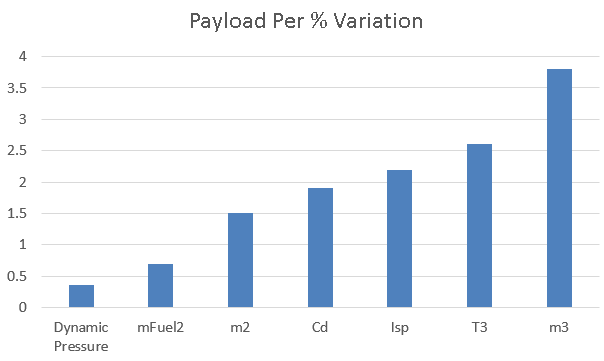
\includegraphics[width=0.7\linewidth]{figures/5_Ascent/BarChartRelativePayloadChange}
\caption{\textcolor{red}{improve this pic (see ingos notes)}}
\label{fig:BarChartRelativePayloadChange}
\end{figure}


\textcolor{red}{more detail, relate to energy trade-off}
The design parameters which increase the velocity at SPARTAN-third stage separation do not cause the SPARTAN to pull-up to higher altitude before third stage release, rather the higher velocity is utilised to allow for a lower release angle at the end of the pull-up manoeuvre. The third stage thrust and drag coefficient are the only parameters which have a significant effect on the release altitude, indicating that it is the third stage performance which is primarily driving the pull-up. 

When the velocity at SPARTAN-third stage separation is varied, the magnitude of the velocity variation carries through in similar magnitude to the third stage velocity at circularisation. This indicates that the $\Delta$v of the third stage before circularisation is relatively consistent. However, the benefits of increased velocity at SPARTAN-third stage separation may potentially be offset slightly by an increase in necessary thermal protection mass, though this is beyond the scope of this study.




\section{Summary}


In this chapter, LODESTAR was used to design the trajectory of the rocket-scramjet-rocket multi-stage system. 
A trajectory was simulated in which the SPARTAN stage flies at a constant dynamic pressure, producing \PayloadToOrbitConstq kg of payload-to-orbit. Trajectory optimisation for maximum payload indicates that the optimal scramjet flight path for a system transitioning between separate airbreathing and rocket-powered stages is for the first stage-SPARTAN separation to occur at a higher trajectory angle than in the constant dynamic pressure trajectory, causing the SPARTAN to fly at lower dynamic pressure initially. The SPARTAN exhibits two more altitude raising manoeuvres, one to extend the flight time and ground coverage of the SPARTAN, and finally a pull-up manoeuvre. The optimal pull-up manoeuvre trades off velocity (a decrease of 116.2m/s) for altitude (an increase of 9.48km) and improved flight path angle (an increase of 10.45$^\circ$), when compared to the constant dynamic pressure case. The optimal flight path increases payload mass to heliocentric orbit to \PayloadToOrbitStandard kg (an increase of 16.3\%) compared to a constant dynamic pressure trajectory. The pull up manoeuvre in the payload-optimised trajectory also reduces maximum dynamic pressure experienced by the third stage to 10.8kPa, a decrease of 43.4kPa compared to a trajectory with minimum pull-up, which allows future benefits due to heat shield mass reduction.  

A sensitivity study was conducted, to determine the relative effects of key vehicle design parameters on the optimised trajectory. It was found that the maximum dynamic pressure has a relatively small effect on the payload-to-orbit performance of the launch system, and the negative efficiency effects which are present are likely to be offset by the benefits of lower dynamic pressure flight. 
It was found that the third stage contributes significantly, and that the efficiency of the third stage is the major driving factor of the pull-up manoeuvre. 
